\documentclass[twoside]{book}

% Packages required by doxygen
\usepackage{fixltx2e}
\usepackage{calc}
\usepackage{doxygen}
\usepackage[export]{adjustbox} % also loads graphicx
\usepackage{graphicx}
\usepackage[utf8]{inputenc}
\usepackage{makeidx}
\usepackage{multicol}
\usepackage{multirow}
\PassOptionsToPackage{warn}{textcomp}
\usepackage{textcomp}
\usepackage[nointegrals]{wasysym}
\usepackage[table]{xcolor}

% Font selection
\usepackage[T1]{fontenc}
\usepackage[scaled=.90]{helvet}
\usepackage{courier}
\usepackage{amssymb}
\usepackage{sectsty}
\renewcommand{\familydefault}{\sfdefault}
\allsectionsfont{%
  \fontseries{bc}\selectfont%
  \color{darkgray}%
}
\renewcommand{\DoxyLabelFont}{%
  \fontseries{bc}\selectfont%
  \color{darkgray}%
}
\newcommand{\+}{\discretionary{\mbox{\scriptsize$\hookleftarrow$}}{}{}}

% Page & text layout
\usepackage{geometry}
\geometry{%
  a4paper,%
  top=2.5cm,%
  bottom=2.5cm,%
  left=2.5cm,%
  right=2.5cm%
}
\tolerance=750
\hfuzz=15pt
\hbadness=750
\setlength{\emergencystretch}{15pt}
\setlength{\parindent}{0cm}
\setlength{\parskip}{3ex plus 2ex minus 2ex}
\makeatletter
\renewcommand{\paragraph}{%
  \@startsection{paragraph}{4}{0ex}{-1.0ex}{1.0ex}{%
    \normalfont\normalsize\bfseries\SS@parafont%
  }%
}
\renewcommand{\subparagraph}{%
  \@startsection{subparagraph}{5}{0ex}{-1.0ex}{1.0ex}{%
    \normalfont\normalsize\bfseries\SS@subparafont%
  }%
}
\makeatother

% Headers & footers
\usepackage{fancyhdr}
\pagestyle{fancyplain}
\fancyhead[LE]{\fancyplain{}{\bfseries\thepage}}
\fancyhead[CE]{\fancyplain{}{}}
\fancyhead[RE]{\fancyplain{}{\bfseries\leftmark}}
\fancyhead[LO]{\fancyplain{}{\bfseries\rightmark}}
\fancyhead[CO]{\fancyplain{}{}}
\fancyhead[RO]{\fancyplain{}{\bfseries\thepage}}
\fancyfoot[LE]{\fancyplain{}{}}
\fancyfoot[CE]{\fancyplain{}{}}
\fancyfoot[RE]{\fancyplain{}{\bfseries\scriptsize Generated by Doxygen }}
\fancyfoot[LO]{\fancyplain{}{\bfseries\scriptsize Generated by Doxygen }}
\fancyfoot[CO]{\fancyplain{}{}}
\fancyfoot[RO]{\fancyplain{}{}}
\renewcommand{\footrulewidth}{0.4pt}
\renewcommand{\chaptermark}[1]{%
  \markboth{#1}{}%
}
\renewcommand{\sectionmark}[1]{%
  \markright{\thesection\ #1}%
}

% Indices & bibliography
\usepackage{natbib}
\usepackage[titles]{tocloft}
\setcounter{tocdepth}{3}
\setcounter{secnumdepth}{5}
\makeindex

% Hyperlinks (required, but should be loaded last)
\usepackage{ifpdf}
\ifpdf
  \usepackage[pdftex,pagebackref=true]{hyperref}
\else
  \usepackage[ps2pdf,pagebackref=true]{hyperref}
\fi
\hypersetup{%
  colorlinks=true,%
  linkcolor=blue,%
  citecolor=blue,%
  unicode%
}

% Custom commands
\newcommand{\clearemptydoublepage}{%
  \newpage{\pagestyle{empty}\cleardoublepage}%
}

\usepackage{caption}
\captionsetup{labelsep=space,justification=centering,font={bf},singlelinecheck=off,skip=4pt,position=top}

%===== C O N T E N T S =====

\begin{document}

% Titlepage & ToC
\hypersetup{pageanchor=false,
             bookmarksnumbered=true,
             pdfencoding=unicode
            }
\pagenumbering{alph}
\begin{titlepage}
\vspace*{7cm}
\begin{center}%
{\Large My Project }\\
\vspace*{1cm}
{\large Generated by Doxygen 1.8.14}\\
\end{center}
\end{titlepage}
\clearemptydoublepage
\pagenumbering{roman}
\tableofcontents
\clearemptydoublepage
\pagenumbering{arabic}
\hypersetup{pageanchor=true}

%--- Begin generated contents ---
\chapter{Hierarchical Index}
\section{Class Hierarchy}
This inheritance list is sorted roughly, but not completely, alphabetically\+:\begin{DoxyCompactList}
\item \contentsline{section}{Client}{\pageref{class_client}}{}
\item Input\+Stream\begin{DoxyCompactList}
\item \contentsline{section}{File\+Stream}{\pageref{class_file_stream}}{}
\end{DoxyCompactList}
\item \contentsline{section}{Map\+Reduce\+Interface}{\pageref{interface_map_reduce_interface}}{}
\begin{DoxyCompactList}
\item \contentsline{section}{Mapper}{\pageref{class_mapper}}{}
\end{DoxyCompactList}
\item \contentsline{section}{Metadata}{\pageref{class_metadata}}{}
\item \contentsline{section}{Meta\+File}{\pageref{class_meta_file}}{}
\item \contentsline{section}{Page}{\pageref{class_page}}{}
\item Remote\begin{DoxyCompactList}
\item \contentsline{section}{Chord\+Message\+Interface}{\pageref{interface_chord_message_interface}}{}
\begin{DoxyCompactList}
\item \contentsline{section}{Chord}{\pageref{class_chord}}{}
\end{DoxyCompactList}
\end{DoxyCompactList}
\item Serializable\begin{DoxyCompactList}
\item \contentsline{section}{D\+FS}{\pageref{class_d_f_s}}{}
\item \contentsline{section}{File\+Stream}{\pageref{class_file_stream}}{}
\end{DoxyCompactList}
\item Unicast\+Remote\+Object\begin{DoxyCompactList}
\item \contentsline{section}{Chord}{\pageref{class_chord}}{}
\end{DoxyCompactList}
\item \contentsline{section}{User\+Interface}{\pageref{class_user_interface}}{}
\end{DoxyCompactList}

\chapter{Class Index}
\section{Class List}
Here are the classes, structs, unions and interfaces with brief descriptions\+:\begin{DoxyCompactList}
\item\contentsline{section}{\mbox{\hyperlink{class_chord}{Chord}} }{\pageref{class_chord}}{}
\item\contentsline{section}{\mbox{\hyperlink{interface_chord_message_interface}{Chord\+Message\+Interface}} }{\pageref{interface_chord_message_interface}}{}
\item\contentsline{section}{\mbox{\hyperlink{class_client}{Client}} }{\pageref{class_client}}{}
\item\contentsline{section}{\mbox{\hyperlink{class_d_f_s}{D\+FS}} }{\pageref{class_d_f_s}}{}
\item\contentsline{section}{\mbox{\hyperlink{class_file_stream}{File\+Stream}} }{\pageref{class_file_stream}}{}
\item\contentsline{section}{\mbox{\hyperlink{class_mapper}{Mapper}} }{\pageref{class_mapper}}{}
\item\contentsline{section}{\mbox{\hyperlink{interface_map_reduce_interface}{Map\+Reduce\+Interface}} }{\pageref{interface_map_reduce_interface}}{}
\item\contentsline{section}{\mbox{\hyperlink{class_metadata}{Metadata}} }{\pageref{class_metadata}}{}
\item\contentsline{section}{\mbox{\hyperlink{class_meta_file}{Meta\+File}} }{\pageref{class_meta_file}}{}
\item\contentsline{section}{\mbox{\hyperlink{class_page}{Page}} }{\pageref{class_page}}{}
\item\contentsline{section}{\mbox{\hyperlink{class_user_interface}{User\+Interface}} }{\pageref{class_user_interface}}{}
\end{DoxyCompactList}

\chapter{Class Documentation}
\hypertarget{class_chord}{}\section{Chord Class Reference}
\label{class_chord}\index{Chord@{Chord}}
Inheritance diagram for Chord\+:\begin{figure}[H]
\begin{center}
\leavevmode
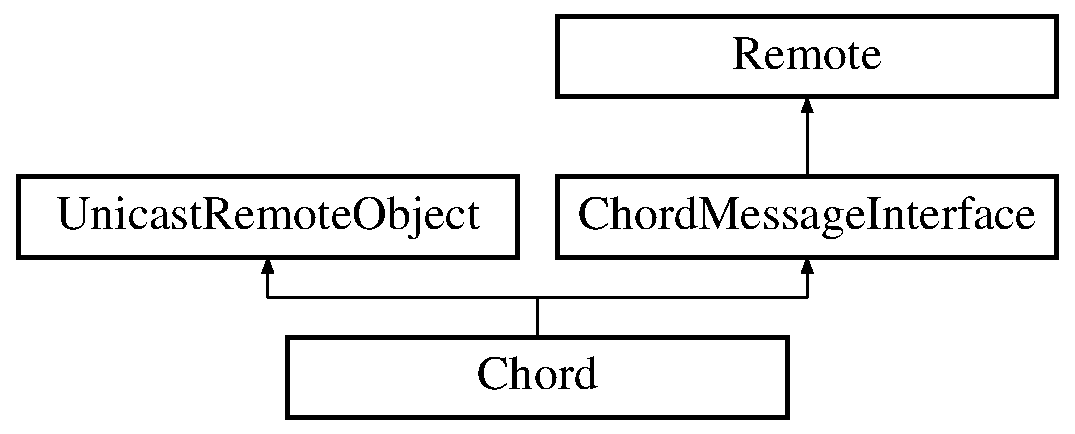
\includegraphics[height=3.000000cm]{class_chord}
\end{center}
\end{figure}
\subsection*{Public Member Functions}
\begin{DoxyCompactItemize}
\item 
Boolean \mbox{\hyperlink{class_chord_aa0b073bf26ea53ee4c36749b5bde4935}{is\+Key\+In\+Semi\+Close\+Interval}} (long key, long key1, long key2)
\item 
Boolean \mbox{\hyperlink{class_chord_a68c9c3d06da58a6a32aa536751d6a221}{is\+Key\+In\+Open\+Interval}} (long key, long key1, long key2)
\item 
void \mbox{\hyperlink{class_chord_a9eb609c00b8f2eddb6e59981d2ff0963}{put}} (long guid\+Object, \mbox{\hyperlink{class_file_stream}{File\+Stream}} stream)  throws Remote\+Exception 
\item 
\mbox{\hyperlink{class_file_stream}{File\+Stream}} \mbox{\hyperlink{class_chord_af273d965e3657c05bd7edcc9f956da23}{get}} (long guid\+Object)  throws Remote\+Exception
\item 
void \mbox{\hyperlink{class_chord_a8bc6bdc9f92665955ae6907f15cc7ea6}{delete}} (long guid\+Object)  throws Remote\+Exception 
\item 
long \mbox{\hyperlink{class_chord_a3dfb600d109b7d23459a3353af0274a9}{get\+Id}} ()  throws Remote\+Exception 
\item 
boolean \mbox{\hyperlink{class_chord_a0a677ced19cc0cb5afd2a695977aeb95}{is\+Alive}} ()  throws Remote\+Exception 
\item 
\mbox{\hyperlink{interface_chord_message_interface}{Chord\+Message\+Interface}} \mbox{\hyperlink{class_chord_a3f1aadce3820e808c80662bb61a58e34}{get\+Predecessor}} ()  throws Remote\+Exception 
\item 
\mbox{\hyperlink{interface_chord_message_interface}{Chord\+Message\+Interface}} \mbox{\hyperlink{class_chord_a7e354ea388d048d4910fa28b182ebe9f}{locate\+Successor}} (long key)  throws Remote\+Exception 
\item 
\mbox{\hyperlink{interface_chord_message_interface}{Chord\+Message\+Interface}} \mbox{\hyperlink{class_chord_aecd3971877558c3b1290bd49d7576ab0}{closest\+Preceding\+Node}} (long key)  throws Remote\+Exception 
\item 
void \mbox{\hyperlink{class_chord_ace0b8d2768590d7527af155c6573cae7}{join\+Ring}} (String ip, int port)  throws Remote\+Exception 
\item 
void \mbox{\hyperlink{class_chord_a65c855dc1d8c6a82545899cb823dba2e}{finding\+Next\+Successor}} ()
\item 
void \mbox{\hyperlink{class_chord_a8a4b7a1cd88cb3f607ada0629f2ff2dd}{stabilize}} ()
\item 
void \mbox{\hyperlink{class_chord_a4de8b8464782dd96d88deeb35b2f27a2}{notify}} (\mbox{\hyperlink{interface_chord_message_interface}{Chord\+Message\+Interface}} j)  throws Remote\+Exception 
\item 
void \mbox{\hyperlink{class_chord_a02763f74bbd986baa7e6567bf9dc3c95}{fix\+Fingers}} ()
\item 
void \mbox{\hyperlink{class_chord_a530b2ab58c9f4026dadf4293c38c4450}{check\+Predecessor}} ()
\item 
Map$<$ Long, String $>$ \mbox{\hyperlink{class_chord_a2439783b411fe026b15a78ba6aeeb95f}{get\+B\+Reduce}} ()
\item 
void \mbox{\hyperlink{class_chord_a14ffe65b5fed6f1e10c5957fe6b9202a}{empty\+Reduce}} ()
\item 
\mbox{\hyperlink{class_chord_a6e4b3112b0268455fd599c57b5479791}{Chord}} (int port, long guid)  throws Remote\+Exception 
\item 
void \mbox{\hyperlink{class_chord_a20d48291de1f865e57a65852e95f7a5e}{set\+Working\+Peer}} (Long page)  throws Remote\+Exception
\item 
void \mbox{\hyperlink{class_chord_a0cc3d82d5173771fcbadb2ee6895d0f8}{complete\+Peer}} (Long page, Long n)  throws Remote\+Exception
\item 
Boolean \mbox{\hyperlink{class_chord_ad34d2c26167785d5d2ff741478367d03}{is\+Phase\+Completed}} ()  throws I\+O\+Exception
\item 
void \mbox{\hyperlink{class_chord_a8fef132c3b9323e35e6bca15153eda3e}{reduce\+Context}} (Long source, \mbox{\hyperlink{interface_map_reduce_interface}{Map\+Reduce\+Interface}} reducer, \mbox{\hyperlink{interface_chord_message_interface}{Chord\+Message\+Interface}} context)  throws Remote\+Exception     
\item 
void \mbox{\hyperlink{class_chord_a6fe57e7be47f45c0be7dfb59c23bb231}{map\+Context}} (Long page, \mbox{\hyperlink{interface_map_reduce_interface}{Map\+Reduce\+Interface}} mapper, \mbox{\hyperlink{interface_chord_message_interface}{Chord\+Message\+Interface}} context)  throws Remote\+Exception, I\+O\+Exception, Exception      
\item 
void \mbox{\hyperlink{class_chord_ad762227086fe020a1eeee133a8262b0d}{emit\+Map}} (Long key, String value)  throws Remote\+Exception     
\item 
void \mbox{\hyperlink{class_chord_af6d622a628500037eec2c4aee5274d40}{emit\+Reduce}} (Long key, String value)  throws Remote\+Exception     
\end{DoxyCompactItemize}
\subsection*{Static Public Attributes}
\begin{DoxyCompactItemize}
\item 
\mbox{\Hypertarget{class_chord_a864e0b4011dc157c78a06dd951c6d9ac}\label{class_chord_a864e0b4011dc157c78a06dd951c6d9ac}} 
static final int {\bfseries M} = 2
\end{DoxyCompactItemize}


\subsection{Constructor \& Destructor Documentation}
\mbox{\Hypertarget{class_chord_a6e4b3112b0268455fd599c57b5479791}\label{class_chord_a6e4b3112b0268455fd599c57b5479791}} 
\index{Chord@{Chord}!Chord@{Chord}}
\index{Chord@{Chord}!Chord@{Chord}}
\subsubsection{\texorpdfstring{Chord()}{Chord()}}
{\footnotesize\ttfamily Chord.\+Chord (\begin{DoxyParamCaption}\item[{int}]{port,  }\item[{long}]{guid }\end{DoxyParamCaption}) throws Remote\+Exception\hspace{0.3cm}{\ttfamily [inline]}}

Constructor for the \mbox{\hyperlink{class_chord}{Chord}} class 
\begin{DoxyParams}{Parameters}
{\em port} & \\
\hline
{\em guid} & \\
\hline
\end{DoxyParams}

\begin{DoxyExceptions}{Exceptions}
{\em Remote\+Exception} & \\
\hline
\end{DoxyExceptions}


\subsection{Member Function Documentation}
\mbox{\Hypertarget{class_chord_a530b2ab58c9f4026dadf4293c38c4450}\label{class_chord_a530b2ab58c9f4026dadf4293c38c4450}} 
\index{Chord@{Chord}!check\+Predecessor@{check\+Predecessor}}
\index{check\+Predecessor@{check\+Predecessor}!Chord@{Chord}}
\subsubsection{\texorpdfstring{check\+Predecessor()}{checkPredecessor()}}
{\footnotesize\ttfamily void Chord.\+check\+Predecessor (\begin{DoxyParamCaption}{ }\end{DoxyParamCaption})\hspace{0.3cm}{\ttfamily [inline]}}

Checks if there is a predecessor preceding \mbox{\Hypertarget{class_chord_aecd3971877558c3b1290bd49d7576ab0}\label{class_chord_aecd3971877558c3b1290bd49d7576ab0}} 
\index{Chord@{Chord}!closest\+Preceding\+Node@{closest\+Preceding\+Node}}
\index{closest\+Preceding\+Node@{closest\+Preceding\+Node}!Chord@{Chord}}
\subsubsection{\texorpdfstring{closest\+Preceding\+Node()}{closestPrecedingNode()}}
{\footnotesize\ttfamily \mbox{\hyperlink{interface_chord_message_interface}{Chord\+Message\+Interface}} Chord.\+closest\+Preceding\+Node (\begin{DoxyParamCaption}\item[{long}]{key }\end{DoxyParamCaption}) throws Remote\+Exception\hspace{0.3cm}{\ttfamily [inline]}}

Returns the node closest to the client 

Implements \mbox{\hyperlink{interface_chord_message_interface}{Chord\+Message\+Interface}}.

\mbox{\Hypertarget{class_chord_a0cc3d82d5173771fcbadb2ee6895d0f8}\label{class_chord_a0cc3d82d5173771fcbadb2ee6895d0f8}} 
\index{Chord@{Chord}!complete\+Peer@{complete\+Peer}}
\index{complete\+Peer@{complete\+Peer}!Chord@{Chord}}
\subsubsection{\texorpdfstring{complete\+Peer()}{completePeer()}}
{\footnotesize\ttfamily void Chord.\+complete\+Peer (\begin{DoxyParamCaption}\item[{Long}]{page,  }\item[{Long}]{n }\end{DoxyParamCaption}) throws Remote\+Exception\hspace{0.3cm}{\ttfamily [inline]}}

Completes the peer connection 

Implements \mbox{\hyperlink{interface_chord_message_interface}{Chord\+Message\+Interface}}.

\mbox{\Hypertarget{class_chord_a8bc6bdc9f92665955ae6907f15cc7ea6}\label{class_chord_a8bc6bdc9f92665955ae6907f15cc7ea6}} 
\index{Chord@{Chord}!delete@{delete}}
\index{delete@{delete}!Chord@{Chord}}
\subsubsection{\texorpdfstring{delete()}{delete()}}
{\footnotesize\ttfamily void Chord.\+delete (\begin{DoxyParamCaption}\item[{long}]{guid\+Object }\end{DoxyParamCaption}) throws Remote\+Exception\hspace{0.3cm}{\ttfamily [inline]}}

Deletes a file posted in the file system 

Implements \mbox{\hyperlink{interface_chord_message_interface}{Chord\+Message\+Interface}}.

\mbox{\Hypertarget{class_chord_ad762227086fe020a1eeee133a8262b0d}\label{class_chord_ad762227086fe020a1eeee133a8262b0d}} 
\index{Chord@{Chord}!emit\+Map@{emit\+Map}}
\index{emit\+Map@{emit\+Map}!Chord@{Chord}}
\subsubsection{\texorpdfstring{emit\+Map()}{emitMap()}}
{\footnotesize\ttfamily void Chord.\+emit\+Map (\begin{DoxyParamCaption}\item[{Long}]{key,  }\item[{String}]{value }\end{DoxyParamCaption}) throws Remote\+Exception\hspace{0.3cm}{\ttfamily [inline]}}

Updates the B\+Map with the results of the mapping phase 

Implements \mbox{\hyperlink{interface_chord_message_interface}{Chord\+Message\+Interface}}.

\mbox{\Hypertarget{class_chord_af6d622a628500037eec2c4aee5274d40}\label{class_chord_af6d622a628500037eec2c4aee5274d40}} 
\index{Chord@{Chord}!emit\+Reduce@{emit\+Reduce}}
\index{emit\+Reduce@{emit\+Reduce}!Chord@{Chord}}
\subsubsection{\texorpdfstring{emit\+Reduce()}{emitReduce()}}
{\footnotesize\ttfamily void Chord.\+emit\+Reduce (\begin{DoxyParamCaption}\item[{Long}]{key,  }\item[{String}]{value }\end{DoxyParamCaption}) throws Remote\+Exception\hspace{0.3cm}{\ttfamily [inline]}}

Updates the peers with the results of the reduce phase 

Implements \mbox{\hyperlink{interface_chord_message_interface}{Chord\+Message\+Interface}}.

\mbox{\Hypertarget{class_chord_a14ffe65b5fed6f1e10c5957fe6b9202a}\label{class_chord_a14ffe65b5fed6f1e10c5957fe6b9202a}} 
\index{Chord@{Chord}!empty\+Reduce@{empty\+Reduce}}
\index{empty\+Reduce@{empty\+Reduce}!Chord@{Chord}}
\subsubsection{\texorpdfstring{empty\+Reduce()}{emptyReduce()}}
{\footnotesize\ttfamily void Chord.\+empty\+Reduce (\begin{DoxyParamCaption}{ }\end{DoxyParamCaption})\hspace{0.3cm}{\ttfamily [inline]}}

Clears the reduce method 

Implements \mbox{\hyperlink{interface_chord_message_interface}{Chord\+Message\+Interface}}.

\mbox{\Hypertarget{class_chord_a65c855dc1d8c6a82545899cb823dba2e}\label{class_chord_a65c855dc1d8c6a82545899cb823dba2e}} 
\index{Chord@{Chord}!finding\+Next\+Successor@{finding\+Next\+Successor}}
\index{finding\+Next\+Successor@{finding\+Next\+Successor}!Chord@{Chord}}
\subsubsection{\texorpdfstring{finding\+Next\+Successor()}{findingNextSuccessor()}}
{\footnotesize\ttfamily void Chord.\+finding\+Next\+Successor (\begin{DoxyParamCaption}{ }\end{DoxyParamCaption})\hspace{0.3cm}{\ttfamily [inline]}}

Returns the successor that is next in the ring \mbox{\Hypertarget{class_chord_a02763f74bbd986baa7e6567bf9dc3c95}\label{class_chord_a02763f74bbd986baa7e6567bf9dc3c95}} 
\index{Chord@{Chord}!fix\+Fingers@{fix\+Fingers}}
\index{fix\+Fingers@{fix\+Fingers}!Chord@{Chord}}
\subsubsection{\texorpdfstring{fix\+Fingers()}{fixFingers()}}
{\footnotesize\ttfamily void Chord.\+fix\+Fingers (\begin{DoxyParamCaption}{ }\end{DoxyParamCaption})\hspace{0.3cm}{\ttfamily [inline]}}

Stabilizes the fingers \mbox{\Hypertarget{class_chord_af273d965e3657c05bd7edcc9f956da23}\label{class_chord_af273d965e3657c05bd7edcc9f956da23}} 
\index{Chord@{Chord}!get@{get}}
\index{get@{get}!Chord@{Chord}}
\subsubsection{\texorpdfstring{get()}{get()}}
{\footnotesize\ttfamily \mbox{\hyperlink{class_file_stream}{File\+Stream}} Chord.\+get (\begin{DoxyParamCaption}\item[{long}]{guid\+Object }\end{DoxyParamCaption}) throws Remote\+Exception\hspace{0.3cm}{\ttfamily [inline]}}

Returns a file posted in the file system. 

Implements \mbox{\hyperlink{interface_chord_message_interface}{Chord\+Message\+Interface}}.

\mbox{\Hypertarget{class_chord_a2439783b411fe026b15a78ba6aeeb95f}\label{class_chord_a2439783b411fe026b15a78ba6aeeb95f}} 
\index{Chord@{Chord}!get\+B\+Reduce@{get\+B\+Reduce}}
\index{get\+B\+Reduce@{get\+B\+Reduce}!Chord@{Chord}}
\subsubsection{\texorpdfstring{get\+B\+Reduce()}{getBReduce()}}
{\footnotesize\ttfamily Map$<$Long, String$>$ Chord.\+get\+B\+Reduce (\begin{DoxyParamCaption}{ }\end{DoxyParamCaption})\hspace{0.3cm}{\ttfamily [inline]}}

Getter method for B\+Reduce 

Implements \mbox{\hyperlink{interface_chord_message_interface}{Chord\+Message\+Interface}}.

\mbox{\Hypertarget{class_chord_a3dfb600d109b7d23459a3353af0274a9}\label{class_chord_a3dfb600d109b7d23459a3353af0274a9}} 
\index{Chord@{Chord}!get\+Id@{get\+Id}}
\index{get\+Id@{get\+Id}!Chord@{Chord}}
\subsubsection{\texorpdfstring{get\+Id()}{getId()}}
{\footnotesize\ttfamily long Chord.\+get\+Id (\begin{DoxyParamCaption}{ }\end{DoxyParamCaption}) throws Remote\+Exception\hspace{0.3cm}{\ttfamily [inline]}}

Getter method for guid 

Implements \mbox{\hyperlink{interface_chord_message_interface}{Chord\+Message\+Interface}}.

\mbox{\Hypertarget{class_chord_a3f1aadce3820e808c80662bb61a58e34}\label{class_chord_a3f1aadce3820e808c80662bb61a58e34}} 
\index{Chord@{Chord}!get\+Predecessor@{get\+Predecessor}}
\index{get\+Predecessor@{get\+Predecessor}!Chord@{Chord}}
\subsubsection{\texorpdfstring{get\+Predecessor()}{getPredecessor()}}
{\footnotesize\ttfamily \mbox{\hyperlink{interface_chord_message_interface}{Chord\+Message\+Interface}} Chord.\+get\+Predecessor (\begin{DoxyParamCaption}{ }\end{DoxyParamCaption}) throws Remote\+Exception\hspace{0.3cm}{\ttfamily [inline]}}

Getter method for Chordmessage\+Interface 

Implements \mbox{\hyperlink{interface_chord_message_interface}{Chord\+Message\+Interface}}.

\mbox{\Hypertarget{class_chord_a0a677ced19cc0cb5afd2a695977aeb95}\label{class_chord_a0a677ced19cc0cb5afd2a695977aeb95}} 
\index{Chord@{Chord}!is\+Alive@{is\+Alive}}
\index{is\+Alive@{is\+Alive}!Chord@{Chord}}
\subsubsection{\texorpdfstring{is\+Alive()}{isAlive()}}
{\footnotesize\ttfamily boolean Chord.\+is\+Alive (\begin{DoxyParamCaption}{ }\end{DoxyParamCaption}) throws Remote\+Exception\hspace{0.3cm}{\ttfamily [inline]}}

Returns true if the process is still executing 

Implements \mbox{\hyperlink{interface_chord_message_interface}{Chord\+Message\+Interface}}.

\mbox{\Hypertarget{class_chord_a68c9c3d06da58a6a32aa536751d6a221}\label{class_chord_a68c9c3d06da58a6a32aa536751d6a221}} 
\index{Chord@{Chord}!is\+Key\+In\+Open\+Interval@{is\+Key\+In\+Open\+Interval}}
\index{is\+Key\+In\+Open\+Interval@{is\+Key\+In\+Open\+Interval}!Chord@{Chord}}
\subsubsection{\texorpdfstring{is\+Key\+In\+Open\+Interval()}{isKeyInOpenInterval()}}
{\footnotesize\ttfamily Boolean Chord.\+is\+Key\+In\+Open\+Interval (\begin{DoxyParamCaption}\item[{long}]{key,  }\item[{long}]{key1,  }\item[{long}]{key2 }\end{DoxyParamCaption})\hspace{0.3cm}{\ttfamily [inline]}}

Returns true if the key is determined to be in the open interval. 
\begin{DoxyParams}{Parameters}
{\em key} & \\
\hline
{\em key1} & \\
\hline
{\em key2} & \\
\hline
\end{DoxyParams}
\begin{DoxyReturn}{Returns}

\end{DoxyReturn}
\mbox{\Hypertarget{class_chord_aa0b073bf26ea53ee4c36749b5bde4935}\label{class_chord_aa0b073bf26ea53ee4c36749b5bde4935}} 
\index{Chord@{Chord}!is\+Key\+In\+Semi\+Close\+Interval@{is\+Key\+In\+Semi\+Close\+Interval}}
\index{is\+Key\+In\+Semi\+Close\+Interval@{is\+Key\+In\+Semi\+Close\+Interval}!Chord@{Chord}}
\subsubsection{\texorpdfstring{is\+Key\+In\+Semi\+Close\+Interval()}{isKeyInSemiCloseInterval()}}
{\footnotesize\ttfamily Boolean Chord.\+is\+Key\+In\+Semi\+Close\+Interval (\begin{DoxyParamCaption}\item[{long}]{key,  }\item[{long}]{key1,  }\item[{long}]{key2 }\end{DoxyParamCaption})\hspace{0.3cm}{\ttfamily [inline]}}

Returns true if the key is determined to be in the interval, false otherwise. 
\begin{DoxyParams}{Parameters}
{\em key} & \\
\hline
{\em key1} & \\
\hline
{\em key2} & \\
\hline
\end{DoxyParams}
\begin{DoxyReturn}{Returns}

\end{DoxyReturn}
\mbox{\Hypertarget{class_chord_ad34d2c26167785d5d2ff741478367d03}\label{class_chord_ad34d2c26167785d5d2ff741478367d03}} 
\index{Chord@{Chord}!is\+Phase\+Completed@{is\+Phase\+Completed}}
\index{is\+Phase\+Completed@{is\+Phase\+Completed}!Chord@{Chord}}
\subsubsection{\texorpdfstring{is\+Phase\+Completed()}{isPhaseCompleted()}}
{\footnotesize\ttfamily Boolean Chord.\+is\+Phase\+Completed (\begin{DoxyParamCaption}{ }\end{DoxyParamCaption}) throws I\+O\+Exception\hspace{0.3cm}{\ttfamily [inline]}}

Returns true if the phase is completed 

Implements \mbox{\hyperlink{interface_chord_message_interface}{Chord\+Message\+Interface}}.

\mbox{\Hypertarget{class_chord_ace0b8d2768590d7527af155c6573cae7}\label{class_chord_ace0b8d2768590d7527af155c6573cae7}} 
\index{Chord@{Chord}!join\+Ring@{join\+Ring}}
\index{join\+Ring@{join\+Ring}!Chord@{Chord}}
\subsubsection{\texorpdfstring{join\+Ring()}{joinRing()}}
{\footnotesize\ttfamily void Chord.\+join\+Ring (\begin{DoxyParamCaption}\item[{String}]{ip,  }\item[{int}]{port }\end{DoxyParamCaption}) throws Remote\+Exception\hspace{0.3cm}{\ttfamily [inline]}}

Creates a connection to the ring in the distributed file system 

Implements \mbox{\hyperlink{interface_chord_message_interface}{Chord\+Message\+Interface}}.

\mbox{\Hypertarget{class_chord_a7e354ea388d048d4910fa28b182ebe9f}\label{class_chord_a7e354ea388d048d4910fa28b182ebe9f}} 
\index{Chord@{Chord}!locate\+Successor@{locate\+Successor}}
\index{locate\+Successor@{locate\+Successor}!Chord@{Chord}}
\subsubsection{\texorpdfstring{locate\+Successor()}{locateSuccessor()}}
{\footnotesize\ttfamily \mbox{\hyperlink{interface_chord_message_interface}{Chord\+Message\+Interface}} Chord.\+locate\+Successor (\begin{DoxyParamCaption}\item[{long}]{key }\end{DoxyParamCaption}) throws Remote\+Exception\hspace{0.3cm}{\ttfamily [inline]}}

Returns the peer closest to the client 

Implements \mbox{\hyperlink{interface_chord_message_interface}{Chord\+Message\+Interface}}.

\mbox{\Hypertarget{class_chord_a6fe57e7be47f45c0be7dfb59c23bb231}\label{class_chord_a6fe57e7be47f45c0be7dfb59c23bb231}} 
\index{Chord@{Chord}!map\+Context@{map\+Context}}
\index{map\+Context@{map\+Context}!Chord@{Chord}}
\subsubsection{\texorpdfstring{map\+Context()}{mapContext()}}
{\footnotesize\ttfamily void Chord.\+map\+Context (\begin{DoxyParamCaption}\item[{Long}]{page,  }\item[{\mbox{\hyperlink{interface_map_reduce_interface}{Map\+Reduce\+Interface}}}]{mapper,  }\item[{\mbox{\hyperlink{interface_chord_message_interface}{Chord\+Message\+Interface}}}]{context }\end{DoxyParamCaption}) throws Remote\+Exception, I\+O\+Exception, Exception\hspace{0.3cm}{\ttfamily [inline]}}

Executes the map phase of Map\+Reduce 

Implements \mbox{\hyperlink{interface_chord_message_interface}{Chord\+Message\+Interface}}.

\mbox{\Hypertarget{class_chord_a4de8b8464782dd96d88deeb35b2f27a2}\label{class_chord_a4de8b8464782dd96d88deeb35b2f27a2}} 
\index{Chord@{Chord}!notify@{notify}}
\index{notify@{notify}!Chord@{Chord}}
\subsubsection{\texorpdfstring{notify()}{notify()}}
{\footnotesize\ttfamily void Chord.\+notify (\begin{DoxyParamCaption}\item[{\mbox{\hyperlink{interface_chord_message_interface}{Chord\+Message\+Interface}}}]{j }\end{DoxyParamCaption}) throws Remote\+Exception\hspace{0.3cm}{\ttfamily [inline]}}

Sends a message to all of the other peers in the network 

Implements \mbox{\hyperlink{interface_chord_message_interface}{Chord\+Message\+Interface}}.

\mbox{\Hypertarget{class_chord_a9eb609c00b8f2eddb6e59981d2ff0963}\label{class_chord_a9eb609c00b8f2eddb6e59981d2ff0963}} 
\index{Chord@{Chord}!put@{put}}
\index{put@{put}!Chord@{Chord}}
\subsubsection{\texorpdfstring{put()}{put()}}
{\footnotesize\ttfamily void Chord.\+put (\begin{DoxyParamCaption}\item[{long}]{guid\+Object,  }\item[{\mbox{\hyperlink{class_file_stream}{File\+Stream}}}]{stream }\end{DoxyParamCaption}) throws Remote\+Exception\hspace{0.3cm}{\ttfamily [inline]}}

Posts a file to the file system 

Implements \mbox{\hyperlink{interface_chord_message_interface}{Chord\+Message\+Interface}}.

\mbox{\Hypertarget{class_chord_a8fef132c3b9323e35e6bca15153eda3e}\label{class_chord_a8fef132c3b9323e35e6bca15153eda3e}} 
\index{Chord@{Chord}!reduce\+Context@{reduce\+Context}}
\index{reduce\+Context@{reduce\+Context}!Chord@{Chord}}
\subsubsection{\texorpdfstring{reduce\+Context()}{reduceContext()}}
{\footnotesize\ttfamily void Chord.\+reduce\+Context (\begin{DoxyParamCaption}\item[{Long}]{source,  }\item[{\mbox{\hyperlink{interface_map_reduce_interface}{Map\+Reduce\+Interface}}}]{reducer,  }\item[{\mbox{\hyperlink{interface_chord_message_interface}{Chord\+Message\+Interface}}}]{context }\end{DoxyParamCaption}) throws Remote\+Exception\hspace{0.3cm}{\ttfamily [inline]}}

Part of the reduce phase of Map\+Reduce, reduces the context 

Implements \mbox{\hyperlink{interface_chord_message_interface}{Chord\+Message\+Interface}}.

\mbox{\Hypertarget{class_chord_a20d48291de1f865e57a65852e95f7a5e}\label{class_chord_a20d48291de1f865e57a65852e95f7a5e}} 
\index{Chord@{Chord}!set\+Working\+Peer@{set\+Working\+Peer}}
\index{set\+Working\+Peer@{set\+Working\+Peer}!Chord@{Chord}}
\subsubsection{\texorpdfstring{set\+Working\+Peer()}{setWorkingPeer()}}
{\footnotesize\ttfamily void Chord.\+set\+Working\+Peer (\begin{DoxyParamCaption}\item[{Long}]{page }\end{DoxyParamCaption}) throws Remote\+Exception\hspace{0.3cm}{\ttfamily [inline]}}

Setter method for the set 

Implements \mbox{\hyperlink{interface_chord_message_interface}{Chord\+Message\+Interface}}.

\mbox{\Hypertarget{class_chord_a8a4b7a1cd88cb3f607ada0629f2ff2dd}\label{class_chord_a8a4b7a1cd88cb3f607ada0629f2ff2dd}} 
\index{Chord@{Chord}!stabilize@{stabilize}}
\index{stabilize@{stabilize}!Chord@{Chord}}
\subsubsection{\texorpdfstring{stabilize()}{stabilize()}}
{\footnotesize\ttfamily void Chord.\+stabilize (\begin{DoxyParamCaption}{ }\end{DoxyParamCaption})\hspace{0.3cm}{\ttfamily [inline]}}

Stabilizes the connection 

The documentation for this class was generated from the following file\+:\begin{DoxyCompactItemize}
\item 
Chord.\+java\end{DoxyCompactItemize}

\hypertarget{interface_chord_message_interface}{}\section{Chord\+Message\+Interface Interface Reference}
\label{interface_chord_message_interface}\index{Chord\+Message\+Interface@{Chord\+Message\+Interface}}
Inheritance diagram for Chord\+Message\+Interface\+:\begin{figure}[H]
\begin{center}
\leavevmode
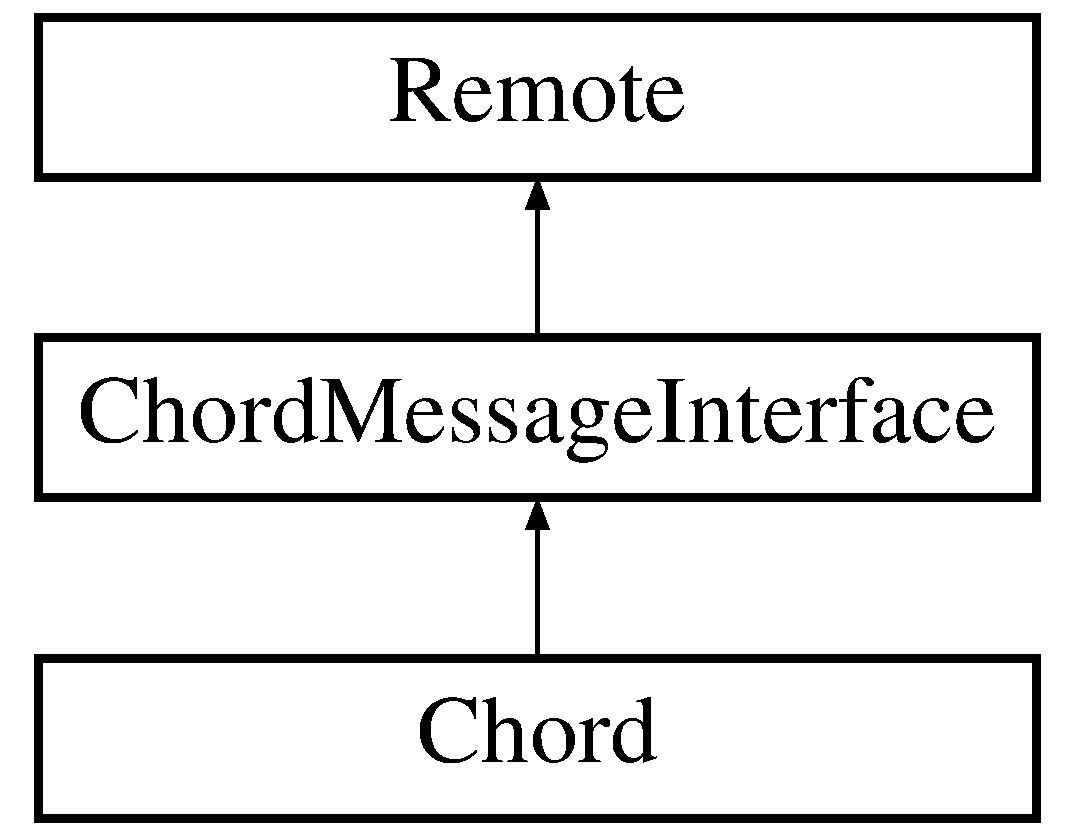
\includegraphics[height=3.000000cm]{interface_chord_message_interface}
\end{center}
\end{figure}
\subsection*{Public Member Functions}
\begin{DoxyCompactItemize}
\item 
\mbox{\Hypertarget{interface_chord_message_interface_ab07c08ba6088ef880eaf4ebae8281c51}\label{interface_chord_message_interface_ab07c08ba6088ef880eaf4ebae8281c51}} 
\mbox{\hyperlink{interface_chord_message_interface}{Chord\+Message\+Interface}} {\bfseries get\+Predecessor} ()  throws Remote\+Exception
\item 
\mbox{\Hypertarget{interface_chord_message_interface_ab7df61ab2cfee0f39206014d7a42b063}\label{interface_chord_message_interface_ab7df61ab2cfee0f39206014d7a42b063}} 
\mbox{\hyperlink{interface_chord_message_interface}{Chord\+Message\+Interface}} {\bfseries locate\+Successor} (long key)  throws Remote\+Exception
\item 
\mbox{\Hypertarget{interface_chord_message_interface_a1d54a4ccd64382455af7dccfd0d6f95f}\label{interface_chord_message_interface_a1d54a4ccd64382455af7dccfd0d6f95f}} 
\mbox{\hyperlink{interface_chord_message_interface}{Chord\+Message\+Interface}} {\bfseries closest\+Preceding\+Node} (long key)  throws Remote\+Exception
\item 
\mbox{\Hypertarget{interface_chord_message_interface_abc5a9483416a6b8ae7330b324869e236}\label{interface_chord_message_interface_abc5a9483416a6b8ae7330b324869e236}} 
void {\bfseries join\+Ring} (String Ip, int port)  throws Remote\+Exception
\item 
\mbox{\Hypertarget{interface_chord_message_interface_abbb77f94541073d79284d35f970e0eb4}\label{interface_chord_message_interface_abbb77f94541073d79284d35f970e0eb4}} 
void {\bfseries notify} (\mbox{\hyperlink{interface_chord_message_interface}{Chord\+Message\+Interface}} j)  throws Remote\+Exception
\item 
\mbox{\Hypertarget{interface_chord_message_interface_a8165b3fb53905e657c70b66223197561}\label{interface_chord_message_interface_a8165b3fb53905e657c70b66223197561}} 
boolean {\bfseries is\+Alive} ()  throws Remote\+Exception
\item 
\mbox{\Hypertarget{interface_chord_message_interface_aaa28e7b91333c557955404ee8d26d65a}\label{interface_chord_message_interface_aaa28e7b91333c557955404ee8d26d65a}} 
long {\bfseries get\+Id} ()  throws Remote\+Exception
\item 
\mbox{\Hypertarget{interface_chord_message_interface_af5cff344c9615be675532d192793e9fd}\label{interface_chord_message_interface_af5cff344c9615be675532d192793e9fd}} 
void {\bfseries put} (long guid\+Object, \mbox{\hyperlink{class_file_stream}{File\+Stream}} input\+Stream)  throws I\+O\+Exception, Remote\+Exception
\item 
\mbox{\Hypertarget{interface_chord_message_interface_a7e5c3d20f8555538899989d1984ce326}\label{interface_chord_message_interface_a7e5c3d20f8555538899989d1984ce326}} 
\mbox{\hyperlink{class_file_stream}{File\+Stream}} {\bfseries get} (long guid\+Object)  throws I\+O\+Exception, Remote\+Exception
\item 
\mbox{\Hypertarget{interface_chord_message_interface_a2bd41258d7f62c5959907e4d3170fc70}\label{interface_chord_message_interface_a2bd41258d7f62c5959907e4d3170fc70}} 
void {\bfseries delete} (long guid\+Object)  throws I\+O\+Exception, Remote\+Exception
\item 
\mbox{\Hypertarget{interface_chord_message_interface_ad3133122275f2af3985da857a55ccffc}\label{interface_chord_message_interface_ad3133122275f2af3985da857a55ccffc}} 
Map$<$ Long, String $>$ {\bfseries get\+B\+Reduce} ()  throws Remote\+Exception
\item 
\mbox{\Hypertarget{interface_chord_message_interface_ab6c24846cee4bedc76ea464b0a115223}\label{interface_chord_message_interface_ab6c24846cee4bedc76ea464b0a115223}} 
void {\bfseries set\+Working\+Peer} (Long page)  throws Remote\+Exception
\item 
\mbox{\Hypertarget{interface_chord_message_interface_ad6e76a8f771acad5a559c991b686fbbc}\label{interface_chord_message_interface_ad6e76a8f771acad5a559c991b686fbbc}} 
void {\bfseries complete\+Peer} (Long page, Long n)  throws Remote\+Exception
\item 
\mbox{\Hypertarget{interface_chord_message_interface_a90bc99e8353719eb8fc11083c5b77220}\label{interface_chord_message_interface_a90bc99e8353719eb8fc11083c5b77220}} 
Boolean {\bfseries is\+Phase\+Completed} ()  throws I\+O\+Exception
\item 
\mbox{\Hypertarget{interface_chord_message_interface_aa04d12dfb770bbc0d0bd63888c20c7cd}\label{interface_chord_message_interface_aa04d12dfb770bbc0d0bd63888c20c7cd}} 
void {\bfseries empty\+Reduce} ()  throws Remote\+Exception
\item 
\mbox{\Hypertarget{interface_chord_message_interface_a21ccb7a25ff36291b3fbdeba29234cd3}\label{interface_chord_message_interface_a21ccb7a25ff36291b3fbdeba29234cd3}} 
void {\bfseries reduce\+Context} (Long source, \mbox{\hyperlink{interface_map_reduce_interface}{Map\+Reduce\+Interface}} reducer, \mbox{\hyperlink{interface_chord_message_interface}{Chord\+Message\+Interface}} context)  throws Remote\+Exception
\item 
\mbox{\Hypertarget{interface_chord_message_interface_a6c0446393624049bded3625f5f41499d}\label{interface_chord_message_interface_a6c0446393624049bded3625f5f41499d}} 
void {\bfseries map\+Context} (Long page, \mbox{\hyperlink{interface_map_reduce_interface}{Map\+Reduce\+Interface}} mapper, \mbox{\hyperlink{interface_chord_message_interface}{Chord\+Message\+Interface}} context)  throws Remote\+Exception, I\+O\+Exception,\+Exception 
\item 
\mbox{\Hypertarget{interface_chord_message_interface_aa6322b11ad33217d05477ed2cef560bb}\label{interface_chord_message_interface_aa6322b11ad33217d05477ed2cef560bb}} 
void {\bfseries emit\+Map} (Long key, String value)  throws Remote\+Exception
\item 
\mbox{\Hypertarget{interface_chord_message_interface_a4c2d3d7293780603d3dc310bba64e631}\label{interface_chord_message_interface_a4c2d3d7293780603d3dc310bba64e631}} 
void {\bfseries emit\+Reduce} (Long page, String value)  throws Remote\+Exception
\end{DoxyCompactItemize}


The documentation for this interface was generated from the following file\+:\begin{DoxyCompactItemize}
\item 
Chord\+Message\+Interface.\+java\end{DoxyCompactItemize}

\hypertarget{class_client}{}\section{Client Class Reference}
\label{class_client}\index{Client@{Client}}
\subsection*{Public Member Functions}
\begin{DoxyCompactItemize}
\item 
\mbox{\hyperlink{class_client_a1862ab048047a5917b5e6a01bf38b78e}{Client}} (int port)  throws Exception 
\item 
void \mbox{\hyperlink{class_client_a3da0518f6e8503b0b669af247ddfcf62}{hello}} ()
\end{DoxyCompactItemize}
\subsection*{Static Public Member Functions}
\begin{DoxyCompactItemize}
\item 
static void \mbox{\hyperlink{class_client_ac4219c51358857184ceeb023ada3d8ae}{main}} (String args\mbox{[}$\,$\mbox{]})  throws Exception     
\end{DoxyCompactItemize}


\subsection{Constructor \& Destructor Documentation}
\mbox{\Hypertarget{class_client_a1862ab048047a5917b5e6a01bf38b78e}\label{class_client_a1862ab048047a5917b5e6a01bf38b78e}} 
\index{Client@{Client}!Client@{Client}}
\index{Client@{Client}!Client@{Client}}
\subsubsection{\texorpdfstring{Client()}{Client()}}
{\footnotesize\ttfamily Client.\+Client (\begin{DoxyParamCaption}\item[{int}]{port }\end{DoxyParamCaption}) throws Exception\hspace{0.3cm}{\ttfamily [inline]}}

Constructor for the client class 
\begin{DoxyParams}{Parameters}
{\em port} & \\
\hline
\end{DoxyParams}

\begin{DoxyExceptions}{Exceptions}
{\em Exception} & \\
\hline
\end{DoxyExceptions}


\subsection{Member Function Documentation}
\mbox{\Hypertarget{class_client_a3da0518f6e8503b0b669af247ddfcf62}\label{class_client_a3da0518f6e8503b0b669af247ddfcf62}} 
\index{Client@{Client}!hello@{hello}}
\index{hello@{hello}!Client@{Client}}
\subsubsection{\texorpdfstring{hello()}{hello()}}
{\footnotesize\ttfamily void Client.\+hello (\begin{DoxyParamCaption}{ }\end{DoxyParamCaption})\hspace{0.3cm}{\ttfamily [inline]}}

Test method to print out a message to the console \mbox{\Hypertarget{class_client_ac4219c51358857184ceeb023ada3d8ae}\label{class_client_ac4219c51358857184ceeb023ada3d8ae}} 
\index{Client@{Client}!main@{main}}
\index{main@{main}!Client@{Client}}
\subsubsection{\texorpdfstring{main()}{main()}}
{\footnotesize\ttfamily static void Client.\+main (\begin{DoxyParamCaption}\item[{String}]{args\mbox{[}$\,$\mbox{]} }\end{DoxyParamCaption}) throws Exception\hspace{0.3cm}{\ttfamily [inline]}, {\ttfamily [static]}}

Whenever a client is instantiated, it\textquotesingle{}ll run an instance of the client? Create three clients, and join two of them (overheard) 
\begin{DoxyParams}{Parameters}
{\em args} & \\
\hline
\end{DoxyParams}

\begin{DoxyExceptions}{Exceptions}
{\em Exception} & \\
\hline
\end{DoxyExceptions}


The documentation for this class was generated from the following file\+:\begin{DoxyCompactItemize}
\item 
Client.\+java\end{DoxyCompactItemize}

\hypertarget{class_d_f_s}{}\section{D\+FS Class Reference}
\label{class_d_f_s}\index{D\+FS@{D\+FS}}
Inheritance diagram for D\+FS\+:\begin{figure}[H]
\begin{center}
\leavevmode
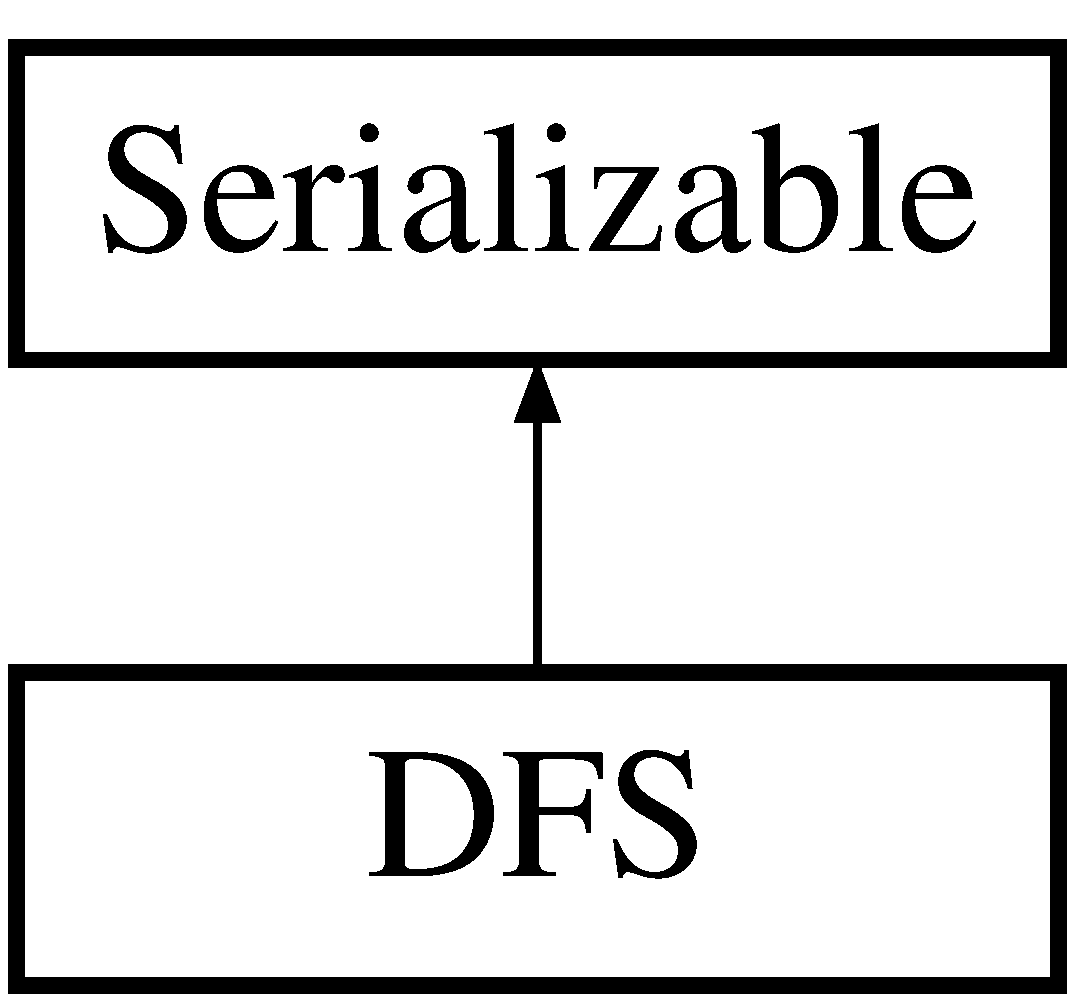
\includegraphics[height=2.000000cm]{class_d_f_s}
\end{center}
\end{figure}
\subsection*{Public Member Functions}
\begin{DoxyCompactItemize}
\item 
\mbox{\hyperlink{class_d_f_s_ad863806217afcce82e64f5d7d4c124ad}{D\+FS}} (int port)  throws Exception     
\item 
void \mbox{\hyperlink{class_d_f_s_a2b7fc8baa8a13aef60da87bde16eb0b3}{set\+Guid}} (long Guid)
\item 
long \mbox{\hyperlink{class_d_f_s_a95f46c984fa3cdd15c03e60c43e54eac}{get\+G\+U\+ID}} ()
\item 
String \mbox{\hyperlink{class_d_f_s_a7024a402890d96dc2cbbc05645a869c8}{get\+String\+Of\+Files}} ()
\item 
void \mbox{\hyperlink{class_d_f_s_a0b41c089ddb9531824556a982e3548eb}{set\+String\+Of\+Files}} (String string\+To\+Concatenate)
\item 
void \mbox{\hyperlink{class_d_f_s_a21222612b26b908c380b73e1e5912a03}{join}} (String ip, int port)  throws Exception 
\item 
\mbox{\hyperlink{class_metadata}{Metadata}} \mbox{\hyperlink{class_d_f_s_a05df5c4a73e10460c29b14b46642eb8a}{read\+Meta\+Data}} ()  throws Exception, Remote\+Exception 
\item 
void \mbox{\hyperlink{class_d_f_s_a2fceb11bdd1e270a4aabcbf9c0dd4339}{write\+Meta\+Data}} (\mbox{\hyperlink{class_metadata}{Metadata}} metadata)  throws Exception 
\item 
Gson \mbox{\hyperlink{class_d_f_s_abdcb090af2467b8a2cfe9ab55b3d9cea}{get\+Gson\+Object}} ()
\item 
void \mbox{\hyperlink{class_d_f_s_ac44bf8288f4423fc87370b97f95f07c1}{touch}} (String file\+Name)  throws Exception 
\item 
String \mbox{\hyperlink{class_d_f_s_a753e09aab8e500f333585f1a6ee865e1}{ls}} ()  throws Exception 
\item 
void \mbox{\hyperlink{class_d_f_s_a7b0d44e11c6176a71d040919b6fe1d96}{mv}} (String old\+Name, String new\+Name)  throws Exception 
\item 
void \mbox{\hyperlink{class_d_f_s_afa4df78a9af4f942cd878afc329b98e1}{delete}} (String file\+Name)  throws Exception 
\item 
\mbox{\hyperlink{class_file_stream}{File\+Stream}} \mbox{\hyperlink{class_d_f_s_a2fe4f98b6e0dede1c97d67bbb5c77df1}{read}} (String file\+Name, int page\+Number)  throws Exception 
\item 
\mbox{\hyperlink{class_file_stream}{File\+Stream}} \mbox{\hyperlink{class_d_f_s_a86ed64f3b14dc0c0d878dbcb1ca1cfa9}{tail}} (String file\+Name)  throws Exception     
\item 
\mbox{\hyperlink{class_file_stream}{File\+Stream}} \mbox{\hyperlink{class_d_f_s_a73915159a4290c3832635b6c4338ff7e}{head}} (String file\+Name)  throws Exception     
\item 
void \mbox{\hyperlink{class_d_f_s_ab2e55db638f5d15efabd544d9a3c4a5f}{append}} (String filename, String local\+File)  throws Exception     
\item 
void \mbox{\hyperlink{class_d_f_s_a51479394a5d22157cc1ee1244d294d00}{run\+Map\+Reduce}} (String filename)  throws Exception     
\item 
void \mbox{\hyperlink{class_d_f_s_a8de3017e98033a0a43c9832fcc15f797}{create\+Page}} (\mbox{\hyperlink{interface_chord_message_interface}{Chord\+Message\+Interface}} context, \mbox{\hyperlink{class_d_f_s}{D\+FS}} \mbox{\hyperlink{class_d_f_s}{D\+FS}}, String name)  throws Exception    
\item 
void \mbox{\hyperlink{class_d_f_s_a6144b8f9a96198128d178badde49d8dc}{append2}} (String filename, Map$<$ Long, String $>$ temp\+Reduce)  throws Exception     
\end{DoxyCompactItemize}


\subsection{Constructor \& Destructor Documentation}
\mbox{\Hypertarget{class_d_f_s_ad863806217afcce82e64f5d7d4c124ad}\label{class_d_f_s_ad863806217afcce82e64f5d7d4c124ad}} 
\index{D\+FS@{D\+FS}!D\+FS@{D\+FS}}
\index{D\+FS@{D\+FS}!D\+FS@{D\+FS}}
\subsubsection{\texorpdfstring{D\+F\+S()}{DFS()}}
{\footnotesize\ttfamily D\+F\+S.\+D\+FS (\begin{DoxyParamCaption}\item[{int}]{port }\end{DoxyParamCaption}) throws Exception\hspace{0.3cm}{\ttfamily [inline]}}

Constructor for the \mbox{\hyperlink{class_d_f_s}{D\+FS}} class. Takes an integer as the port number. 
\begin{DoxyParams}{Parameters}
{\em port} & \\
\hline
\end{DoxyParams}

\begin{DoxyExceptions}{Exceptions}
{\em Exception} & \\
\hline
\end{DoxyExceptions}


\subsection{Member Function Documentation}
\mbox{\Hypertarget{class_d_f_s_ab2e55db638f5d15efabd544d9a3c4a5f}\label{class_d_f_s_ab2e55db638f5d15efabd544d9a3c4a5f}} 
\index{D\+FS@{D\+FS}!append@{append}}
\index{append@{append}!D\+FS@{D\+FS}}
\subsubsection{\texorpdfstring{append()}{append()}}
{\footnotesize\ttfamily void D\+F\+S.\+append (\begin{DoxyParamCaption}\item[{String}]{filename,  }\item[{String}]{local\+File }\end{DoxyParamCaption}) throws Exception\hspace{0.3cm}{\ttfamily [inline]}}

Adds a new file to the end of the array of files in the metadata. 
\begin{DoxyParams}{Parameters}
{\em filename} & \\
\hline
{\em filepath} & \\
\hline
\end{DoxyParams}

\begin{DoxyExceptions}{Exceptions}
{\em Exception} & \\
\hline
\end{DoxyExceptions}
\mbox{\Hypertarget{class_d_f_s_a6144b8f9a96198128d178badde49d8dc}\label{class_d_f_s_a6144b8f9a96198128d178badde49d8dc}} 
\index{D\+FS@{D\+FS}!append2@{append2}}
\index{append2@{append2}!D\+FS@{D\+FS}}
\subsubsection{\texorpdfstring{append2()}{append2()}}
{\footnotesize\ttfamily void D\+F\+S.\+append2 (\begin{DoxyParamCaption}\item[{String}]{filename,  }\item[{Map$<$ Long, String $>$}]{temp\+Reduce }\end{DoxyParamCaption}) throws Exception\hspace{0.3cm}{\ttfamily [inline]}}

Appends a page to a file. 
\begin{DoxyParams}{Parameters}
{\em filename} & \\
\hline
{\em temp\+Reduce} & \\
\hline
\end{DoxyParams}

\begin{DoxyExceptions}{Exceptions}
{\em Exception} & \\
\hline
\end{DoxyExceptions}
\mbox{\Hypertarget{class_d_f_s_a8de3017e98033a0a43c9832fcc15f797}\label{class_d_f_s_a8de3017e98033a0a43c9832fcc15f797}} 
\index{D\+FS@{D\+FS}!create\+Page@{create\+Page}}
\index{create\+Page@{create\+Page}!D\+FS@{D\+FS}}
\subsubsection{\texorpdfstring{create\+Page()}{createPage()}}
{\footnotesize\ttfamily void D\+F\+S.\+create\+Page (\begin{DoxyParamCaption}\item[{\mbox{\hyperlink{interface_chord_message_interface}{Chord\+Message\+Interface}}}]{context,  }\item[{\mbox{\hyperlink{class_d_f_s}{D\+FS}}}]{D\+FS,  }\item[{String}]{name }\end{DoxyParamCaption}) throws Exception\hspace{0.3cm}{\ttfamily [inline]}}

Creates a page to be added to a file. 
\begin{DoxyParams}{Parameters}
{\em context} & \\
\hline
{\em \mbox{\hyperlink{class_d_f_s}{D\+FS}}} & \\
\hline
{\em name} & \\
\hline
\end{DoxyParams}

\begin{DoxyExceptions}{Exceptions}
{\em Exception} & \\
\hline
\end{DoxyExceptions}
\mbox{\Hypertarget{class_d_f_s_afa4df78a9af4f942cd878afc329b98e1}\label{class_d_f_s_afa4df78a9af4f942cd878afc329b98e1}} 
\index{D\+FS@{D\+FS}!delete@{delete}}
\index{delete@{delete}!D\+FS@{D\+FS}}
\subsubsection{\texorpdfstring{delete()}{delete()}}
{\footnotesize\ttfamily void D\+F\+S.\+delete (\begin{DoxyParamCaption}\item[{String}]{file\+Name }\end{DoxyParamCaption}) throws Exception\hspace{0.3cm}{\ttfamily [inline]}}

Deletes a file and all of its pages from the metadata. 
\begin{DoxyParams}{Parameters}
{\em file\+Name} & \\
\hline
\end{DoxyParams}

\begin{DoxyExceptions}{Exceptions}
{\em Exception} & \\
\hline
\end{DoxyExceptions}
\mbox{\Hypertarget{class_d_f_s_abdcb090af2467b8a2cfe9ab55b3d9cea}\label{class_d_f_s_abdcb090af2467b8a2cfe9ab55b3d9cea}} 
\index{D\+FS@{D\+FS}!get\+Gson\+Object@{get\+Gson\+Object}}
\index{get\+Gson\+Object@{get\+Gson\+Object}!D\+FS@{D\+FS}}
\subsubsection{\texorpdfstring{get\+Gson\+Object()}{getGsonObject()}}
{\footnotesize\ttfamily Gson D\+F\+S.\+get\+Gson\+Object (\begin{DoxyParamCaption}{ }\end{DoxyParamCaption})\hspace{0.3cm}{\ttfamily [inline]}}

Getter method for the gson \begin{DoxyReturn}{Returns}

\end{DoxyReturn}
\mbox{\Hypertarget{class_d_f_s_a95f46c984fa3cdd15c03e60c43e54eac}\label{class_d_f_s_a95f46c984fa3cdd15c03e60c43e54eac}} 
\index{D\+FS@{D\+FS}!get\+G\+U\+ID@{get\+G\+U\+ID}}
\index{get\+G\+U\+ID@{get\+G\+U\+ID}!D\+FS@{D\+FS}}
\subsubsection{\texorpdfstring{get\+G\+U\+I\+D()}{getGUID()}}
{\footnotesize\ttfamily long D\+F\+S.\+get\+G\+U\+ID (\begin{DoxyParamCaption}{ }\end{DoxyParamCaption})\hspace{0.3cm}{\ttfamily [inline]}}

Getter method for guid \begin{DoxyReturn}{Returns}

\end{DoxyReturn}
\mbox{\Hypertarget{class_d_f_s_a7024a402890d96dc2cbbc05645a869c8}\label{class_d_f_s_a7024a402890d96dc2cbbc05645a869c8}} 
\index{D\+FS@{D\+FS}!get\+String\+Of\+Files@{get\+String\+Of\+Files}}
\index{get\+String\+Of\+Files@{get\+String\+Of\+Files}!D\+FS@{D\+FS}}
\subsubsection{\texorpdfstring{get\+String\+Of\+Files()}{getStringOfFiles()}}
{\footnotesize\ttfamily String D\+F\+S.\+get\+String\+Of\+Files (\begin{DoxyParamCaption}{ }\end{DoxyParamCaption})\hspace{0.3cm}{\ttfamily [inline]}}

Getter method for list\+Of\+Files \begin{DoxyReturn}{Returns}

\end{DoxyReturn}
\mbox{\Hypertarget{class_d_f_s_a73915159a4290c3832635b6c4338ff7e}\label{class_d_f_s_a73915159a4290c3832635b6c4338ff7e}} 
\index{D\+FS@{D\+FS}!head@{head}}
\index{head@{head}!D\+FS@{D\+FS}}
\subsubsection{\texorpdfstring{head()}{head()}}
{\footnotesize\ttfamily \mbox{\hyperlink{class_file_stream}{File\+Stream}} D\+F\+S.\+head (\begin{DoxyParamCaption}\item[{String}]{file\+Name }\end{DoxyParamCaption}) throws Exception\hspace{0.3cm}{\ttfamily [inline]}}

Returns the first page of the file in the metadata. 
\begin{DoxyParams}{Parameters}
{\em file\+Name} & \\
\hline
\end{DoxyParams}
\begin{DoxyReturn}{Returns}

\end{DoxyReturn}

\begin{DoxyExceptions}{Exceptions}
{\em Exception} & \\
\hline
\end{DoxyExceptions}
\mbox{\Hypertarget{class_d_f_s_a21222612b26b908c380b73e1e5912a03}\label{class_d_f_s_a21222612b26b908c380b73e1e5912a03}} 
\index{D\+FS@{D\+FS}!join@{join}}
\index{join@{join}!D\+FS@{D\+FS}}
\subsubsection{\texorpdfstring{join()}{join()}}
{\footnotesize\ttfamily void D\+F\+S.\+join (\begin{DoxyParamCaption}\item[{String}]{ip,  }\item[{int}]{port }\end{DoxyParamCaption}) throws Exception\hspace{0.3cm}{\ttfamily [inline]}}

Method to join a process to a \mbox{\hyperlink{class_chord}{Chord}} network 
\begin{DoxyParams}{Parameters}
{\em ip} & IP address of the machine\textquotesingle{}s network you wish to join \\
\hline
{\em port} & of the network \\
\hline
\end{DoxyParams}

\begin{DoxyExceptions}{Exceptions}
{\em Exception} & \\
\hline
\end{DoxyExceptions}
\mbox{\Hypertarget{class_d_f_s_a753e09aab8e500f333585f1a6ee865e1}\label{class_d_f_s_a753e09aab8e500f333585f1a6ee865e1}} 
\index{D\+FS@{D\+FS}!ls@{ls}}
\index{ls@{ls}!D\+FS@{D\+FS}}
\subsubsection{\texorpdfstring{ls()}{ls()}}
{\footnotesize\ttfamily String D\+F\+S.\+ls (\begin{DoxyParamCaption}{ }\end{DoxyParamCaption}) throws Exception\hspace{0.3cm}{\ttfamily [inline]}}

Returns a list of the files in the metadata in the form of a string. \begin{DoxyReturn}{Returns}

\end{DoxyReturn}

\begin{DoxyExceptions}{Exceptions}
{\em Exception} & \\
\hline
\end{DoxyExceptions}
\mbox{\Hypertarget{class_d_f_s_a7b0d44e11c6176a71d040919b6fe1d96}\label{class_d_f_s_a7b0d44e11c6176a71d040919b6fe1d96}} 
\index{D\+FS@{D\+FS}!mv@{mv}}
\index{mv@{mv}!D\+FS@{D\+FS}}
\subsubsection{\texorpdfstring{mv()}{mv()}}
{\footnotesize\ttfamily void D\+F\+S.\+mv (\begin{DoxyParamCaption}\item[{String}]{old\+Name,  }\item[{String}]{new\+Name }\end{DoxyParamCaption}) throws Exception\hspace{0.3cm}{\ttfamily [inline]}}

Renames the metadata object. 
\begin{DoxyParams}{Parameters}
{\em old\+Name} & \\
\hline
{\em new\+Name} & \\
\hline
\end{DoxyParams}

\begin{DoxyExceptions}{Exceptions}
{\em Exception} & \\
\hline
\end{DoxyExceptions}
\mbox{\Hypertarget{class_d_f_s_a2fe4f98b6e0dede1c97d67bbb5c77df1}\label{class_d_f_s_a2fe4f98b6e0dede1c97d67bbb5c77df1}} 
\index{D\+FS@{D\+FS}!read@{read}}
\index{read@{read}!D\+FS@{D\+FS}}
\subsubsection{\texorpdfstring{read()}{read()}}
{\footnotesize\ttfamily \mbox{\hyperlink{class_file_stream}{File\+Stream}} D\+F\+S.\+read (\begin{DoxyParamCaption}\item[{String}]{file\+Name,  }\item[{int}]{page\+Number }\end{DoxyParamCaption}) throws Exception\hspace{0.3cm}{\ttfamily [inline]}}

Returns a page from a file from the metadata in the form of a \mbox{\hyperlink{class_file_stream}{File\+Stream}}. 
\begin{DoxyParams}{Parameters}
{\em file\+Name} & \\
\hline
{\em page\+Number} & \\
\hline
\end{DoxyParams}
\begin{DoxyReturn}{Returns}

\end{DoxyReturn}

\begin{DoxyExceptions}{Exceptions}
{\em Exception} & \\
\hline
\end{DoxyExceptions}
\mbox{\Hypertarget{class_d_f_s_a05df5c4a73e10460c29b14b46642eb8a}\label{class_d_f_s_a05df5c4a73e10460c29b14b46642eb8a}} 
\index{D\+FS@{D\+FS}!read\+Meta\+Data@{read\+Meta\+Data}}
\index{read\+Meta\+Data@{read\+Meta\+Data}!D\+FS@{D\+FS}}
\subsubsection{\texorpdfstring{read\+Meta\+Data()}{readMetaData()}}
{\footnotesize\ttfamily \mbox{\hyperlink{class_metadata}{Metadata}} D\+F\+S.\+read\+Meta\+Data (\begin{DoxyParamCaption}{ }\end{DoxyParamCaption}) throws Exception, Remote\+Exception\hspace{0.3cm}{\ttfamily [inline]}}

Reads the metadata object from the File System \begin{DoxyReturn}{Returns}
\mbox{\hyperlink{class_metadata}{Metadata}} 
\end{DoxyReturn}

\begin{DoxyExceptions}{Exceptions}
{\em Exception} & \\
\hline
{\em Remote\+Exception} & \\
\hline
\end{DoxyExceptions}
\mbox{\Hypertarget{class_d_f_s_a51479394a5d22157cc1ee1244d294d00}\label{class_d_f_s_a51479394a5d22157cc1ee1244d294d00}} 
\index{D\+FS@{D\+FS}!run\+Map\+Reduce@{run\+Map\+Reduce}}
\index{run\+Map\+Reduce@{run\+Map\+Reduce}!D\+FS@{D\+FS}}
\subsubsection{\texorpdfstring{run\+Map\+Reduce()}{runMapReduce()}}
{\footnotesize\ttfamily void D\+F\+S.\+run\+Map\+Reduce (\begin{DoxyParamCaption}\item[{String}]{filename }\end{DoxyParamCaption}) throws Exception\hspace{0.3cm}{\ttfamily [inline]}}

Executes the map reduce process 
\begin{DoxyParams}{Parameters}
{\em filename} & \\
\hline
\end{DoxyParams}

\begin{DoxyExceptions}{Exceptions}
{\em Exception} & \\
\hline
\end{DoxyExceptions}
\mbox{\Hypertarget{class_d_f_s_a2b7fc8baa8a13aef60da87bde16eb0b3}\label{class_d_f_s_a2b7fc8baa8a13aef60da87bde16eb0b3}} 
\index{D\+FS@{D\+FS}!set\+Guid@{set\+Guid}}
\index{set\+Guid@{set\+Guid}!D\+FS@{D\+FS}}
\subsubsection{\texorpdfstring{set\+Guid()}{setGuid()}}
{\footnotesize\ttfamily void D\+F\+S.\+set\+Guid (\begin{DoxyParamCaption}\item[{long}]{Guid }\end{DoxyParamCaption})\hspace{0.3cm}{\ttfamily [inline]}}

Setter method for guid. 
\begin{DoxyParams}{Parameters}
{\em Guid} & \\
\hline
\end{DoxyParams}
\mbox{\Hypertarget{class_d_f_s_a0b41c089ddb9531824556a982e3548eb}\label{class_d_f_s_a0b41c089ddb9531824556a982e3548eb}} 
\index{D\+FS@{D\+FS}!set\+String\+Of\+Files@{set\+String\+Of\+Files}}
\index{set\+String\+Of\+Files@{set\+String\+Of\+Files}!D\+FS@{D\+FS}}
\subsubsection{\texorpdfstring{set\+String\+Of\+Files()}{setStringOfFiles()}}
{\footnotesize\ttfamily void D\+F\+S.\+set\+String\+Of\+Files (\begin{DoxyParamCaption}\item[{String}]{string\+To\+Concatenate }\end{DoxyParamCaption})\hspace{0.3cm}{\ttfamily [inline]}}

Setter method for list\+Of\+Files 
\begin{DoxyParams}{Parameters}
{\em string\+To\+Concatenate} & \\
\hline
\end{DoxyParams}
\mbox{\Hypertarget{class_d_f_s_a86ed64f3b14dc0c0d878dbcb1ca1cfa9}\label{class_d_f_s_a86ed64f3b14dc0c0d878dbcb1ca1cfa9}} 
\index{D\+FS@{D\+FS}!tail@{tail}}
\index{tail@{tail}!D\+FS@{D\+FS}}
\subsubsection{\texorpdfstring{tail()}{tail()}}
{\footnotesize\ttfamily \mbox{\hyperlink{class_file_stream}{File\+Stream}} D\+F\+S.\+tail (\begin{DoxyParamCaption}\item[{String}]{file\+Name }\end{DoxyParamCaption}) throws Exception\hspace{0.3cm}{\ttfamily [inline]}}

Returns the last page of a file in the metadata in the form of a Filestream. 
\begin{DoxyParams}{Parameters}
{\em file\+Name} & \\
\hline
\end{DoxyParams}
\begin{DoxyReturn}{Returns}
Filestream 
\end{DoxyReturn}

\begin{DoxyExceptions}{Exceptions}
{\em Exception} & \\
\hline
\end{DoxyExceptions}
\mbox{\Hypertarget{class_d_f_s_ac44bf8288f4423fc87370b97f95f07c1}\label{class_d_f_s_ac44bf8288f4423fc87370b97f95f07c1}} 
\index{D\+FS@{D\+FS}!touch@{touch}}
\index{touch@{touch}!D\+FS@{D\+FS}}
\subsubsection{\texorpdfstring{touch()}{touch()}}
{\footnotesize\ttfamily void D\+F\+S.\+touch (\begin{DoxyParamCaption}\item[{String}]{file\+Name }\end{DoxyParamCaption}) throws Exception\hspace{0.3cm}{\ttfamily [inline]}}

Creates a new file with the inputted name into the metadata object. 
\begin{DoxyParams}{Parameters}
{\em file\+Name} & \\
\hline
\end{DoxyParams}

\begin{DoxyExceptions}{Exceptions}
{\em Exception} & \\
\hline
\end{DoxyExceptions}
\mbox{\Hypertarget{class_d_f_s_a2fceb11bdd1e270a4aabcbf9c0dd4339}\label{class_d_f_s_a2fceb11bdd1e270a4aabcbf9c0dd4339}} 
\index{D\+FS@{D\+FS}!write\+Meta\+Data@{write\+Meta\+Data}}
\index{write\+Meta\+Data@{write\+Meta\+Data}!D\+FS@{D\+FS}}
\subsubsection{\texorpdfstring{write\+Meta\+Data()}{writeMetaData()}}
{\footnotesize\ttfamily void D\+F\+S.\+write\+Meta\+Data (\begin{DoxyParamCaption}\item[{\mbox{\hyperlink{class_metadata}{Metadata}}}]{metadata }\end{DoxyParamCaption}) throws Exception\hspace{0.3cm}{\ttfamily [inline]}}

Writes the local files into the File System 
\begin{DoxyParams}{Parameters}
{\em metadata} & \\
\hline
\end{DoxyParams}

\begin{DoxyExceptions}{Exceptions}
{\em Exception} & \\
\hline
\end{DoxyExceptions}


The documentation for this class was generated from the following file\+:\begin{DoxyCompactItemize}
\item 
D\+F\+S.\+java\end{DoxyCompactItemize}

\hypertarget{class_file_stream}{}\section{File\+Stream Class Reference}
\label{class_file_stream}\index{File\+Stream@{File\+Stream}}
Inheritance diagram for File\+Stream\+:\begin{figure}[H]
\begin{center}
\leavevmode
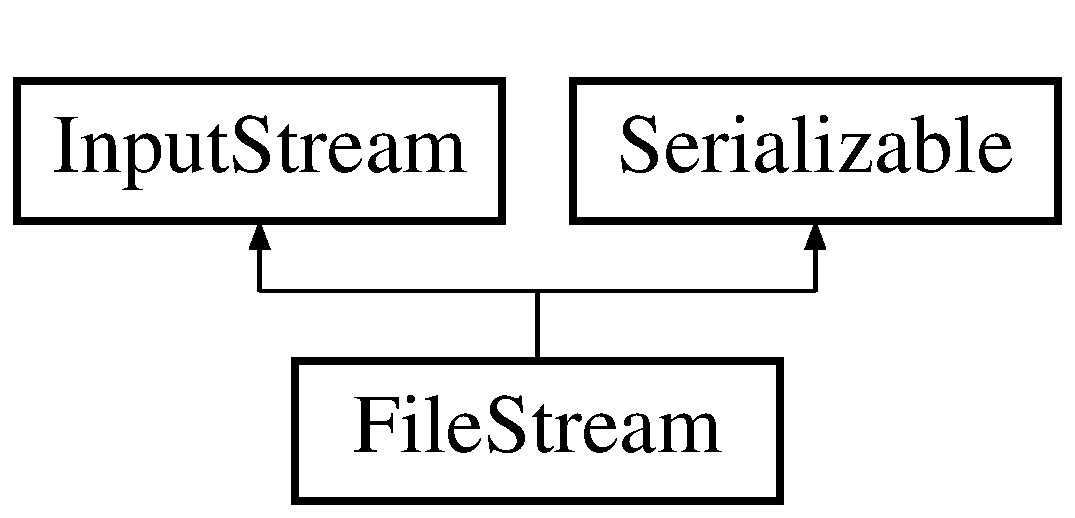
\includegraphics[height=2.000000cm]{class_file_stream}
\end{center}
\end{figure}
\subsection*{Public Member Functions}
\begin{DoxyCompactItemize}
\item 
\mbox{\hyperlink{class_file_stream_a120b1fd6e4c74e93199d063da1c65b98}{File\+Stream}} (String path\+Name)  throws File\+Not\+Found\+Exception, I\+O\+Exception 
\item 
\mbox{\hyperlink{class_file_stream_a69fed4812620e26c3fd23560993bf7b3}{File\+Stream}} (Byte\mbox{[}$\,$\mbox{]} byte\+Array)
\item 
\mbox{\hyperlink{class_file_stream_aa919eed4082491d09520911563d44efd}{File\+Stream}} ()  throws File\+Not\+Found\+Exception    
\item 
int \mbox{\hyperlink{class_file_stream_a7f2ea40eff2241931a4ca971364cd532}{read}} ()  throws I\+O\+Exception 
\item 
int \mbox{\hyperlink{class_file_stream_a7dd240b96afa9e37f9a6bd8e4b99e48b}{available}} ()  throws I\+O\+Exception     
\item 
int \mbox{\hyperlink{class_file_stream_ab8f4d0c94a6c1357c7af77a4121e52fc}{get\+Size}} ()
\item 
String \mbox{\hyperlink{class_file_stream_ab5040ef2d7c336c123902ab493001866}{get\+Path}} ()
\item 
void \mbox{\hyperlink{class_file_stream_a10b53b74a061e2bedc6fadbfaa5660b5}{set\+Path}} (String new\+Path)
\item 
File \mbox{\hyperlink{class_file_stream_a0e12c8a0391372eebb0d444014af6c58}{get\+File}} ()
\item 
void \mbox{\hyperlink{class_file_stream_a0885a5602d71d48e503d6b19ac40bc17}{set\+File}} (File new\+File)
\end{DoxyCompactItemize}


\subsection{Constructor \& Destructor Documentation}
\mbox{\Hypertarget{class_file_stream_a120b1fd6e4c74e93199d063da1c65b98}\label{class_file_stream_a120b1fd6e4c74e93199d063da1c65b98}} 
\index{File\+Stream@{File\+Stream}!File\+Stream@{File\+Stream}}
\index{File\+Stream@{File\+Stream}!File\+Stream@{File\+Stream}}
\subsubsection{\texorpdfstring{File\+Stream()}{FileStream()}\hspace{0.1cm}{\footnotesize\ttfamily [1/3]}}
{\footnotesize\ttfamily File\+Stream.\+File\+Stream (\begin{DoxyParamCaption}\item[{String}]{path\+Name }\end{DoxyParamCaption}) throws File\+Not\+Found\+Exception, I\+O\+Exception\hspace{0.3cm}{\ttfamily [inline]}}

Constructor for the \mbox{\hyperlink{class_file_stream}{File\+Stream}} class 
\begin{DoxyParams}{Parameters}
{\em path\+Name} & \\
\hline
\end{DoxyParams}

\begin{DoxyExceptions}{Exceptions}
{\em File\+Not\+Found\+Exception} & \\
\hline
{\em I\+O\+Exception} & \\
\hline
\end{DoxyExceptions}
\mbox{\Hypertarget{class_file_stream_a69fed4812620e26c3fd23560993bf7b3}\label{class_file_stream_a69fed4812620e26c3fd23560993bf7b3}} 
\index{File\+Stream@{File\+Stream}!File\+Stream@{File\+Stream}}
\index{File\+Stream@{File\+Stream}!File\+Stream@{File\+Stream}}
\subsubsection{\texorpdfstring{File\+Stream()}{FileStream()}\hspace{0.1cm}{\footnotesize\ttfamily [2/3]}}
{\footnotesize\ttfamily File\+Stream.\+File\+Stream (\begin{DoxyParamCaption}\item[{Byte \mbox{[}$\,$\mbox{]}}]{byte\+Array }\end{DoxyParamCaption})\hspace{0.3cm}{\ttfamily [inline]}}

Alternate constructor 
\begin{DoxyParams}{Parameters}
{\em byte\+Array} & \\
\hline
\end{DoxyParams}
\mbox{\Hypertarget{class_file_stream_aa919eed4082491d09520911563d44efd}\label{class_file_stream_aa919eed4082491d09520911563d44efd}} 
\index{File\+Stream@{File\+Stream}!File\+Stream@{File\+Stream}}
\index{File\+Stream@{File\+Stream}!File\+Stream@{File\+Stream}}
\subsubsection{\texorpdfstring{File\+Stream()}{FileStream()}\hspace{0.1cm}{\footnotesize\ttfamily [3/3]}}
{\footnotesize\ttfamily File\+Stream.\+File\+Stream (\begin{DoxyParamCaption}{ }\end{DoxyParamCaption}) throws File\+Not\+Found\+Exception\hspace{0.3cm}{\ttfamily [inline]}}

Alternate constructor 
\begin{DoxyExceptions}{Exceptions}
{\em File\+Not\+Found\+Exception} & \\
\hline
\end{DoxyExceptions}


\subsection{Member Function Documentation}
\mbox{\Hypertarget{class_file_stream_a7dd240b96afa9e37f9a6bd8e4b99e48b}\label{class_file_stream_a7dd240b96afa9e37f9a6bd8e4b99e48b}} 
\index{File\+Stream@{File\+Stream}!available@{available}}
\index{available@{available}!File\+Stream@{File\+Stream}}
\subsubsection{\texorpdfstring{available()}{available()}}
{\footnotesize\ttfamily int File\+Stream.\+available (\begin{DoxyParamCaption}{ }\end{DoxyParamCaption}) throws I\+O\+Exception\hspace{0.3cm}{\ttfamily [inline]}}

Returns the availble space remaining \mbox{\Hypertarget{class_file_stream_a0e12c8a0391372eebb0d444014af6c58}\label{class_file_stream_a0e12c8a0391372eebb0d444014af6c58}} 
\index{File\+Stream@{File\+Stream}!get\+File@{get\+File}}
\index{get\+File@{get\+File}!File\+Stream@{File\+Stream}}
\subsubsection{\texorpdfstring{get\+File()}{getFile()}}
{\footnotesize\ttfamily File File\+Stream.\+get\+File (\begin{DoxyParamCaption}{ }\end{DoxyParamCaption})\hspace{0.3cm}{\ttfamily [inline]}}

Getter method for the file \begin{DoxyReturn}{Returns}

\end{DoxyReturn}
\mbox{\Hypertarget{class_file_stream_ab5040ef2d7c336c123902ab493001866}\label{class_file_stream_ab5040ef2d7c336c123902ab493001866}} 
\index{File\+Stream@{File\+Stream}!get\+Path@{get\+Path}}
\index{get\+Path@{get\+Path}!File\+Stream@{File\+Stream}}
\subsubsection{\texorpdfstring{get\+Path()}{getPath()}}
{\footnotesize\ttfamily String File\+Stream.\+get\+Path (\begin{DoxyParamCaption}{ }\end{DoxyParamCaption})\hspace{0.3cm}{\ttfamily [inline]}}

Getter method for the path \begin{DoxyReturn}{Returns}

\end{DoxyReturn}
\mbox{\Hypertarget{class_file_stream_ab8f4d0c94a6c1357c7af77a4121e52fc}\label{class_file_stream_ab8f4d0c94a6c1357c7af77a4121e52fc}} 
\index{File\+Stream@{File\+Stream}!get\+Size@{get\+Size}}
\index{get\+Size@{get\+Size}!File\+Stream@{File\+Stream}}
\subsubsection{\texorpdfstring{get\+Size()}{getSize()}}
{\footnotesize\ttfamily int File\+Stream.\+get\+Size (\begin{DoxyParamCaption}{ }\end{DoxyParamCaption})\hspace{0.3cm}{\ttfamily [inline]}}

Getter method for the size \begin{DoxyReturn}{Returns}

\end{DoxyReturn}
\mbox{\Hypertarget{class_file_stream_a7f2ea40eff2241931a4ca971364cd532}\label{class_file_stream_a7f2ea40eff2241931a4ca971364cd532}} 
\index{File\+Stream@{File\+Stream}!read@{read}}
\index{read@{read}!File\+Stream@{File\+Stream}}
\subsubsection{\texorpdfstring{read()}{read()}}
{\footnotesize\ttfamily int File\+Stream.\+read (\begin{DoxyParamCaption}{ }\end{DoxyParamCaption}) throws I\+O\+Exception\hspace{0.3cm}{\ttfamily [inline]}}

Reads a file from the filestream \mbox{\Hypertarget{class_file_stream_a0885a5602d71d48e503d6b19ac40bc17}\label{class_file_stream_a0885a5602d71d48e503d6b19ac40bc17}} 
\index{File\+Stream@{File\+Stream}!set\+File@{set\+File}}
\index{set\+File@{set\+File}!File\+Stream@{File\+Stream}}
\subsubsection{\texorpdfstring{set\+File()}{setFile()}}
{\footnotesize\ttfamily void File\+Stream.\+set\+File (\begin{DoxyParamCaption}\item[{File}]{new\+File }\end{DoxyParamCaption})\hspace{0.3cm}{\ttfamily [inline]}}

Setter method for the file \mbox{\Hypertarget{class_file_stream_a10b53b74a061e2bedc6fadbfaa5660b5}\label{class_file_stream_a10b53b74a061e2bedc6fadbfaa5660b5}} 
\index{File\+Stream@{File\+Stream}!set\+Path@{set\+Path}}
\index{set\+Path@{set\+Path}!File\+Stream@{File\+Stream}}
\subsubsection{\texorpdfstring{set\+Path()}{setPath()}}
{\footnotesize\ttfamily void File\+Stream.\+set\+Path (\begin{DoxyParamCaption}\item[{String}]{new\+Path }\end{DoxyParamCaption})\hspace{0.3cm}{\ttfamily [inline]}}

Setter method for the path 
\begin{DoxyParams}{Parameters}
{\em new\+Path} & \\
\hline
\end{DoxyParams}


The documentation for this class was generated from the following file\+:\begin{DoxyCompactItemize}
\item 
File\+Stream.\+java\end{DoxyCompactItemize}

\hypertarget{class_mapper}{}\section{Mapper Class Reference}
\label{class_mapper}\index{Mapper@{Mapper}}
Inheritance diagram for Mapper\+:\begin{figure}[H]
\begin{center}
\leavevmode
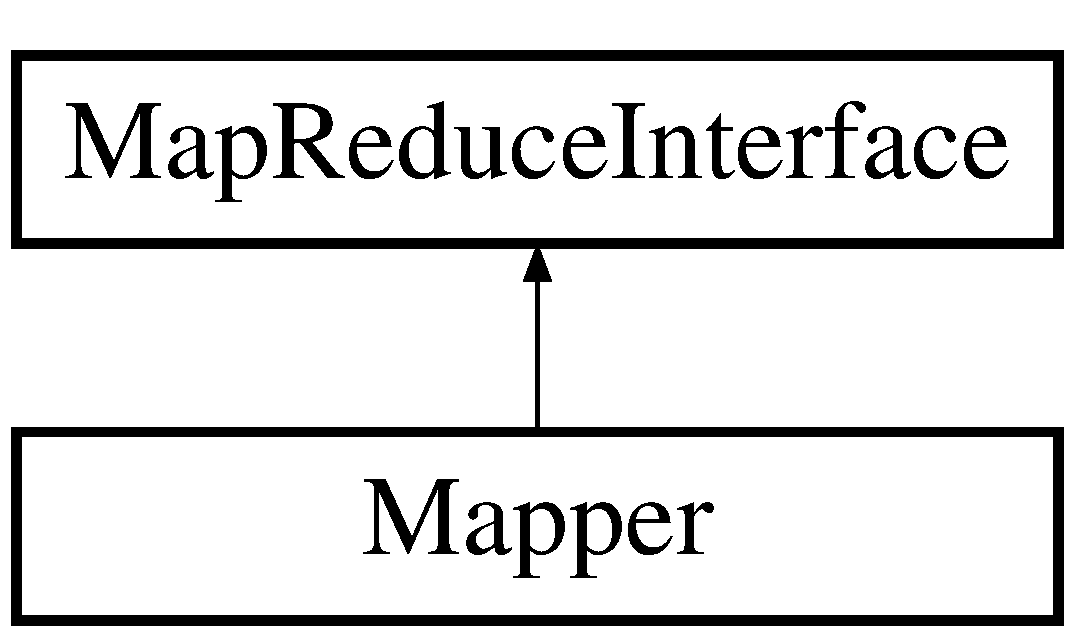
\includegraphics[height=2.000000cm]{class_mapper}
\end{center}
\end{figure}
\subsection*{Public Member Functions}
\begin{DoxyCompactItemize}
\item 
void \mbox{\hyperlink{class_mapper_ad694fe6234676a05e2ee63aec14942c8}{map}} (Long key, String value, \mbox{\hyperlink{interface_chord_message_interface}{Chord\+Message\+Interface}} context)  throws I\+O\+Exception 	
\item 
void \mbox{\hyperlink{class_mapper_a5c6a53e9cd1419e4b5eded401331c2fd}{reduce}} (Long key, List$<$ String $>$ value, \mbox{\hyperlink{interface_chord_message_interface}{Chord\+Message\+Interface}} context)  throws I\+O\+Exception 	
\end{DoxyCompactItemize}


\subsection{Member Function Documentation}
\mbox{\Hypertarget{class_mapper_ad694fe6234676a05e2ee63aec14942c8}\label{class_mapper_ad694fe6234676a05e2ee63aec14942c8}} 
\index{Mapper@{Mapper}!map@{map}}
\index{map@{map}!Mapper@{Mapper}}
\subsubsection{\texorpdfstring{map()}{map()}}
{\footnotesize\ttfamily void Mapper.\+map (\begin{DoxyParamCaption}\item[{Long}]{key,  }\item[{String}]{value,  }\item[{\mbox{\hyperlink{interface_chord_message_interface}{Chord\+Message\+Interface}}}]{context }\end{DoxyParamCaption}) throws I\+O\+Exception\hspace{0.3cm}{\ttfamily [inline]}}

Executes the mapping phase of the chord class. 

Implements \mbox{\hyperlink{interface_map_reduce_interface}{Map\+Reduce\+Interface}}.

\mbox{\Hypertarget{class_mapper_a5c6a53e9cd1419e4b5eded401331c2fd}\label{class_mapper_a5c6a53e9cd1419e4b5eded401331c2fd}} 
\index{Mapper@{Mapper}!reduce@{reduce}}
\index{reduce@{reduce}!Mapper@{Mapper}}
\subsubsection{\texorpdfstring{reduce()}{reduce()}}
{\footnotesize\ttfamily void Mapper.\+reduce (\begin{DoxyParamCaption}\item[{Long}]{key,  }\item[{List$<$ String $>$}]{value,  }\item[{\mbox{\hyperlink{interface_chord_message_interface}{Chord\+Message\+Interface}}}]{context }\end{DoxyParamCaption}) throws I\+O\+Exception\hspace{0.3cm}{\ttfamily [inline]}}

Executes the reduce phase of the chord class 

Implements \mbox{\hyperlink{interface_map_reduce_interface}{Map\+Reduce\+Interface}}.



The documentation for this class was generated from the following file\+:\begin{DoxyCompactItemize}
\item 
Mapper.\+java\end{DoxyCompactItemize}

\hypertarget{interface_map_reduce_interface}{}\section{Map\+Reduce\+Interface Interface Reference}
\label{interface_map_reduce_interface}\index{Map\+Reduce\+Interface@{Map\+Reduce\+Interface}}
Inheritance diagram for Map\+Reduce\+Interface\+:\begin{figure}[H]
\begin{center}
\leavevmode
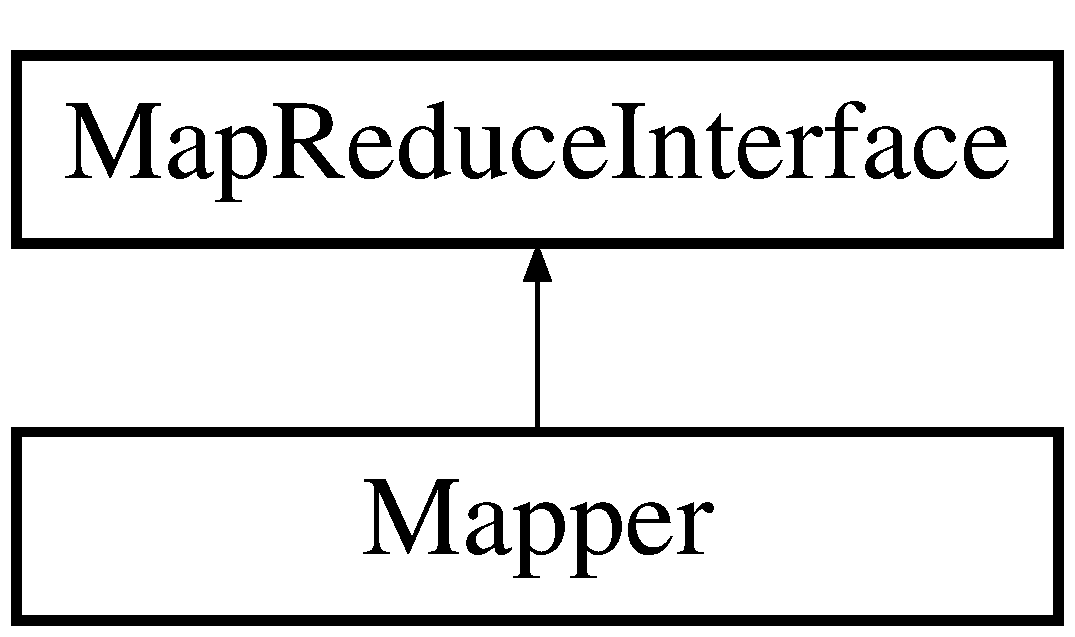
\includegraphics[height=2.000000cm]{interface_map_reduce_interface}
\end{center}
\end{figure}
\subsection*{Public Member Functions}
\begin{DoxyCompactItemize}
\item 
\mbox{\Hypertarget{interface_map_reduce_interface_aceecf9558b0390e89c3995a2711e3f15}\label{interface_map_reduce_interface_aceecf9558b0390e89c3995a2711e3f15}} 
void {\bfseries map} (Long key, String value, \mbox{\hyperlink{interface_chord_message_interface}{Chord\+Message\+Interface}} context)  throws I\+O\+Exception
\item 
\mbox{\Hypertarget{interface_map_reduce_interface_a2824dc60ea3e1415dc01a5d0c6e7b683}\label{interface_map_reduce_interface_a2824dc60ea3e1415dc01a5d0c6e7b683}} 
void {\bfseries reduce} (Long key, List$<$ String $>$ value, \mbox{\hyperlink{interface_chord_message_interface}{Chord\+Message\+Interface}} context)  throws I\+O\+Exception
\end{DoxyCompactItemize}


The documentation for this interface was generated from the following file\+:\begin{DoxyCompactItemize}
\item 
Map\+Reduce\+Interface.\+java\end{DoxyCompactItemize}

\hypertarget{class_metadata}{}\section{Metadata Class Reference}
\label{class_metadata}\index{Metadata@{Metadata}}
\subsection*{Public Member Functions}
\begin{DoxyCompactItemize}
\item 
\mbox{\hyperlink{class_metadata_a05084417d8815ec44e3d70126f31be00}{Metadata}} ()
\item 
void \mbox{\hyperlink{class_metadata_afba93e3d4b961ddcd67b5f2530a9e20d}{change\+Name}} (String old\+Name, String new\+Name)
\item 
String \mbox{\hyperlink{class_metadata_a47932985a21ca5fe3e99726b50c36658}{get\+File\+Names}} ()
\item 
void \mbox{\hyperlink{class_metadata_a67800e2f003cabb15744b86bec38a783}{create\+File}} (String file\+Name)  throws File\+Not\+Found\+Exception, I\+O\+Exception 
\item 
\mbox{\hyperlink{class_meta_file}{Meta\+File}} \mbox{\hyperlink{class_metadata_ae29cb4e7e73fdda5a3649e085863d481}{get\+File}} (String file\+Name)  throws Exception 
\item 
void \mbox{\hyperlink{class_metadata_a84c1111ef377e908c90bf9afb6006e20}{delete}} (String file\+Name)
\item 
void \mbox{\hyperlink{class_metadata_a84c55073051d681405262f85feed7286}{append}} (String name, String local\+File)
\item 
void \mbox{\hyperlink{class_metadata_ad553fd3bd0610354c55d603c64886533}{to\+Json}} ()
\item 
void \mbox{\hyperlink{class_metadata_ab22a1ff2f8390792d6c520be50dd3906}{readfrom\+J\+S\+ON}} ()
\end{DoxyCompactItemize}


\subsection{Constructor \& Destructor Documentation}
\mbox{\Hypertarget{class_metadata_a05084417d8815ec44e3d70126f31be00}\label{class_metadata_a05084417d8815ec44e3d70126f31be00}} 
\index{Metadata@{Metadata}!Metadata@{Metadata}}
\index{Metadata@{Metadata}!Metadata@{Metadata}}
\subsubsection{\texorpdfstring{Metadata()}{Metadata()}}
{\footnotesize\ttfamily Metadata.\+Metadata (\begin{DoxyParamCaption}{ }\end{DoxyParamCaption})\hspace{0.3cm}{\ttfamily [inline]}}

Constructor for the \mbox{\hyperlink{class_metadata}{Metadata}} class 

\subsection{Member Function Documentation}
\mbox{\Hypertarget{class_metadata_a84c55073051d681405262f85feed7286}\label{class_metadata_a84c55073051d681405262f85feed7286}} 
\index{Metadata@{Metadata}!append@{append}}
\index{append@{append}!Metadata@{Metadata}}
\subsubsection{\texorpdfstring{append()}{append()}}
{\footnotesize\ttfamily void Metadata.\+append (\begin{DoxyParamCaption}\item[{String}]{name,  }\item[{String}]{local\+File }\end{DoxyParamCaption})\hspace{0.3cm}{\ttfamily [inline]}}

Appends a file to the metadata 
\begin{DoxyParams}{Parameters}
{\em name} & \\
\hline
{\em local\+File} & \\
\hline
\end{DoxyParams}
\mbox{\Hypertarget{class_metadata_afba93e3d4b961ddcd67b5f2530a9e20d}\label{class_metadata_afba93e3d4b961ddcd67b5f2530a9e20d}} 
\index{Metadata@{Metadata}!change\+Name@{change\+Name}}
\index{change\+Name@{change\+Name}!Metadata@{Metadata}}
\subsubsection{\texorpdfstring{change\+Name()}{changeName()}}
{\footnotesize\ttfamily void Metadata.\+change\+Name (\begin{DoxyParamCaption}\item[{String}]{old\+Name,  }\item[{String}]{new\+Name }\end{DoxyParamCaption})\hspace{0.3cm}{\ttfamily [inline]}}

Sets the metafile\textquotesingle{}s name to a new one 
\begin{DoxyParams}{Parameters}
{\em old\+Name} & \\
\hline
{\em new\+Name} & \\
\hline
\end{DoxyParams}
\mbox{\Hypertarget{class_metadata_a67800e2f003cabb15744b86bec38a783}\label{class_metadata_a67800e2f003cabb15744b86bec38a783}} 
\index{Metadata@{Metadata}!create\+File@{create\+File}}
\index{create\+File@{create\+File}!Metadata@{Metadata}}
\subsubsection{\texorpdfstring{create\+File()}{createFile()}}
{\footnotesize\ttfamily void Metadata.\+create\+File (\begin{DoxyParamCaption}\item[{String}]{file\+Name }\end{DoxyParamCaption}) throws File\+Not\+Found\+Exception, I\+O\+Exception\hspace{0.3cm}{\ttfamily [inline]}}

Creates a file and adds it to the metafile 
\begin{DoxyParams}{Parameters}
{\em file\+Name} & \\
\hline
\end{DoxyParams}

\begin{DoxyExceptions}{Exceptions}
{\em File\+Not\+Found\+Exception} & \\
\hline
{\em I\+O\+Exception} & \\
\hline
\end{DoxyExceptions}
\mbox{\Hypertarget{class_metadata_a84c1111ef377e908c90bf9afb6006e20}\label{class_metadata_a84c1111ef377e908c90bf9afb6006e20}} 
\index{Metadata@{Metadata}!delete@{delete}}
\index{delete@{delete}!Metadata@{Metadata}}
\subsubsection{\texorpdfstring{delete()}{delete()}}
{\footnotesize\ttfamily void Metadata.\+delete (\begin{DoxyParamCaption}\item[{String}]{file\+Name }\end{DoxyParamCaption})\hspace{0.3cm}{\ttfamily [inline]}}

Deletes a file from metadata 
\begin{DoxyParams}{Parameters}
{\em file\+Name} & \\
\hline
\end{DoxyParams}
\mbox{\Hypertarget{class_metadata_ae29cb4e7e73fdda5a3649e085863d481}\label{class_metadata_ae29cb4e7e73fdda5a3649e085863d481}} 
\index{Metadata@{Metadata}!get\+File@{get\+File}}
\index{get\+File@{get\+File}!Metadata@{Metadata}}
\subsubsection{\texorpdfstring{get\+File()}{getFile()}}
{\footnotesize\ttfamily \mbox{\hyperlink{class_meta_file}{Meta\+File}} Metadata.\+get\+File (\begin{DoxyParamCaption}\item[{String}]{file\+Name }\end{DoxyParamCaption}) throws Exception\hspace{0.3cm}{\ttfamily [inline]}}

Returns a specified file 
\begin{DoxyParams}{Parameters}
{\em file\+Name} & \\
\hline
\end{DoxyParams}
\begin{DoxyReturn}{Returns}

\end{DoxyReturn}

\begin{DoxyExceptions}{Exceptions}
{\em Exception} & \\
\hline
\end{DoxyExceptions}
\mbox{\Hypertarget{class_metadata_a47932985a21ca5fe3e99726b50c36658}\label{class_metadata_a47932985a21ca5fe3e99726b50c36658}} 
\index{Metadata@{Metadata}!get\+File\+Names@{get\+File\+Names}}
\index{get\+File\+Names@{get\+File\+Names}!Metadata@{Metadata}}
\subsubsection{\texorpdfstring{get\+File\+Names()}{getFileNames()}}
{\footnotesize\ttfamily String Metadata.\+get\+File\+Names (\begin{DoxyParamCaption}{ }\end{DoxyParamCaption})\hspace{0.3cm}{\ttfamily [inline]}}

Returns a list of all of the file\textquotesingle{}s names \begin{DoxyReturn}{Returns}

\end{DoxyReturn}
\mbox{\Hypertarget{class_metadata_ab22a1ff2f8390792d6c520be50dd3906}\label{class_metadata_ab22a1ff2f8390792d6c520be50dd3906}} 
\index{Metadata@{Metadata}!readfrom\+J\+S\+ON@{readfrom\+J\+S\+ON}}
\index{readfrom\+J\+S\+ON@{readfrom\+J\+S\+ON}!Metadata@{Metadata}}
\subsubsection{\texorpdfstring{readfrom\+J\+S\+O\+N()}{readfromJSON()}}
{\footnotesize\ttfamily void Metadata.\+readfrom\+J\+S\+ON (\begin{DoxyParamCaption}{ }\end{DoxyParamCaption})\hspace{0.3cm}{\ttfamily [inline]}}

converts a json to a string \mbox{\Hypertarget{class_metadata_ad553fd3bd0610354c55d603c64886533}\label{class_metadata_ad553fd3bd0610354c55d603c64886533}} 
\index{Metadata@{Metadata}!to\+Json@{to\+Json}}
\index{to\+Json@{to\+Json}!Metadata@{Metadata}}
\subsubsection{\texorpdfstring{to\+Json()}{toJson()}}
{\footnotesize\ttfamily void Metadata.\+to\+Json (\begin{DoxyParamCaption}{ }\end{DoxyParamCaption})\hspace{0.3cm}{\ttfamily [inline]}}

Converts a string to json 

The documentation for this class was generated from the following file\+:\begin{DoxyCompactItemize}
\item 
Metadata.\+java\end{DoxyCompactItemize}

\hypertarget{class_meta_file}{}\section{Meta\+File Class Reference}
\label{class_meta_file}\index{Meta\+File@{Meta\+File}}
\subsection*{Public Member Functions}
\begin{DoxyCompactItemize}
\item 
\mbox{\hyperlink{class_meta_file_aa0e71eb6d56f1e50c2cf53c321a7b4c0}{Meta\+File}} (String name, int number\+Of\+Pages, int page\+Size, int size, Array\+List$<$ \mbox{\hyperlink{class_page}{Page}} $>$ pages)
\item 
\mbox{\hyperlink{class_meta_file_a66c83b5972fe6b3baf1d5f3e79790890}{Meta\+File}} ()
\item 
String \mbox{\hyperlink{class_meta_file_a7704cca7da5d2e765d70d01562d6f4da}{get\+Name}} ()
\item 
void \mbox{\hyperlink{class_meta_file_ac4abf81a1fb0c5478b13527091345ed5}{set\+Name}} (String new\+Name)
\item 
\mbox{\hyperlink{class_page}{Page}} \mbox{\hyperlink{class_meta_file_a28c7cbf3f8889b484df5b11b99825a4e}{get\+Page}} (int page\+Num)  throws Exception 	
\item 
\mbox{\hyperlink{class_page}{Page}} \mbox{\hyperlink{class_meta_file_adf3ad8347572a056d3a7ae730c120303}{get\+Last\+Page}} ()
\item 
void \mbox{\hyperlink{class_meta_file_a5244a5a75cdf85974ae9cb94b5490a21}{add\+Page}} (\mbox{\hyperlink{class_page}{Page}} page\+Object)
\item 
\mbox{\hyperlink{class_page}{Page}} \mbox{\hyperlink{class_meta_file_a495f8b327a312ebcdd54e7dbfdd98ee5}{get\+First\+Page}} ()
\item 
int \mbox{\hyperlink{class_meta_file_a05c2f305a2e388e3482962321ff7ba7e}{get\+Num\+Of\+Page}} ()
\end{DoxyCompactItemize}


\subsection{Constructor \& Destructor Documentation}
\mbox{\Hypertarget{class_meta_file_aa0e71eb6d56f1e50c2cf53c321a7b4c0}\label{class_meta_file_aa0e71eb6d56f1e50c2cf53c321a7b4c0}} 
\index{Meta\+File@{Meta\+File}!Meta\+File@{Meta\+File}}
\index{Meta\+File@{Meta\+File}!Meta\+File@{Meta\+File}}
\subsubsection{\texorpdfstring{Meta\+File()}{MetaFile()}\hspace{0.1cm}{\footnotesize\ttfamily [1/2]}}
{\footnotesize\ttfamily Meta\+File.\+Meta\+File (\begin{DoxyParamCaption}\item[{String}]{name,  }\item[{int}]{number\+Of\+Pages,  }\item[{int}]{page\+Size,  }\item[{int}]{size,  }\item[{Array\+List$<$ \mbox{\hyperlink{class_page}{Page}} $>$}]{pages }\end{DoxyParamCaption})\hspace{0.3cm}{\ttfamily [inline]}}

Constructor for the Metafile class 
\begin{DoxyParams}{Parameters}
{\em name} & \\
\hline
{\em number\+Of\+Pages} & \\
\hline
{\em page\+Size} & \\
\hline
{\em size} & \\
\hline
{\em pages} & \\
\hline
\end{DoxyParams}
\mbox{\Hypertarget{class_meta_file_a66c83b5972fe6b3baf1d5f3e79790890}\label{class_meta_file_a66c83b5972fe6b3baf1d5f3e79790890}} 
\index{Meta\+File@{Meta\+File}!Meta\+File@{Meta\+File}}
\index{Meta\+File@{Meta\+File}!Meta\+File@{Meta\+File}}
\subsubsection{\texorpdfstring{Meta\+File()}{MetaFile()}\hspace{0.1cm}{\footnotesize\ttfamily [2/2]}}
{\footnotesize\ttfamily Meta\+File.\+Meta\+File (\begin{DoxyParamCaption}{ }\end{DoxyParamCaption})\hspace{0.3cm}{\ttfamily [inline]}}

Alternate constructor for the metafile class 

\subsection{Member Function Documentation}
\mbox{\Hypertarget{class_meta_file_a5244a5a75cdf85974ae9cb94b5490a21}\label{class_meta_file_a5244a5a75cdf85974ae9cb94b5490a21}} 
\index{Meta\+File@{Meta\+File}!add\+Page@{add\+Page}}
\index{add\+Page@{add\+Page}!Meta\+File@{Meta\+File}}
\subsubsection{\texorpdfstring{add\+Page()}{addPage()}}
{\footnotesize\ttfamily void Meta\+File.\+add\+Page (\begin{DoxyParamCaption}\item[{\mbox{\hyperlink{class_page}{Page}}}]{page\+Object }\end{DoxyParamCaption})\hspace{0.3cm}{\ttfamily [inline]}}

Appends a page to a file 
\begin{DoxyParams}{Parameters}
{\em page\+Object} & \\
\hline
\end{DoxyParams}
\mbox{\Hypertarget{class_meta_file_a495f8b327a312ebcdd54e7dbfdd98ee5}\label{class_meta_file_a495f8b327a312ebcdd54e7dbfdd98ee5}} 
\index{Meta\+File@{Meta\+File}!get\+First\+Page@{get\+First\+Page}}
\index{get\+First\+Page@{get\+First\+Page}!Meta\+File@{Meta\+File}}
\subsubsection{\texorpdfstring{get\+First\+Page()}{getFirstPage()}}
{\footnotesize\ttfamily \mbox{\hyperlink{class_page}{Page}} Meta\+File.\+get\+First\+Page (\begin{DoxyParamCaption}{ }\end{DoxyParamCaption})\hspace{0.3cm}{\ttfamily [inline]}}

Returns the first page in the file \begin{DoxyReturn}{Returns}

\end{DoxyReturn}
\mbox{\Hypertarget{class_meta_file_adf3ad8347572a056d3a7ae730c120303}\label{class_meta_file_adf3ad8347572a056d3a7ae730c120303}} 
\index{Meta\+File@{Meta\+File}!get\+Last\+Page@{get\+Last\+Page}}
\index{get\+Last\+Page@{get\+Last\+Page}!Meta\+File@{Meta\+File}}
\subsubsection{\texorpdfstring{get\+Last\+Page()}{getLastPage()}}
{\footnotesize\ttfamily \mbox{\hyperlink{class_page}{Page}} Meta\+File.\+get\+Last\+Page (\begin{DoxyParamCaption}{ }\end{DoxyParamCaption})\hspace{0.3cm}{\ttfamily [inline]}}

Returns the last page in the metafile \begin{DoxyReturn}{Returns}

\end{DoxyReturn}
\mbox{\Hypertarget{class_meta_file_a7704cca7da5d2e765d70d01562d6f4da}\label{class_meta_file_a7704cca7da5d2e765d70d01562d6f4da}} 
\index{Meta\+File@{Meta\+File}!get\+Name@{get\+Name}}
\index{get\+Name@{get\+Name}!Meta\+File@{Meta\+File}}
\subsubsection{\texorpdfstring{get\+Name()}{getName()}}
{\footnotesize\ttfamily String Meta\+File.\+get\+Name (\begin{DoxyParamCaption}{ }\end{DoxyParamCaption})\hspace{0.3cm}{\ttfamily [inline]}}

Getter method for the name \begin{DoxyReturn}{Returns}

\end{DoxyReturn}
\mbox{\Hypertarget{class_meta_file_a05c2f305a2e388e3482962321ff7ba7e}\label{class_meta_file_a05c2f305a2e388e3482962321ff7ba7e}} 
\index{Meta\+File@{Meta\+File}!get\+Num\+Of\+Page@{get\+Num\+Of\+Page}}
\index{get\+Num\+Of\+Page@{get\+Num\+Of\+Page}!Meta\+File@{Meta\+File}}
\subsubsection{\texorpdfstring{get\+Num\+Of\+Page()}{getNumOfPage()}}
{\footnotesize\ttfamily int Meta\+File.\+get\+Num\+Of\+Page (\begin{DoxyParamCaption}{ }\end{DoxyParamCaption})\hspace{0.3cm}{\ttfamily [inline]}}

Returns the index of a page \begin{DoxyReturn}{Returns}

\end{DoxyReturn}
\mbox{\Hypertarget{class_meta_file_a28c7cbf3f8889b484df5b11b99825a4e}\label{class_meta_file_a28c7cbf3f8889b484df5b11b99825a4e}} 
\index{Meta\+File@{Meta\+File}!get\+Page@{get\+Page}}
\index{get\+Page@{get\+Page}!Meta\+File@{Meta\+File}}
\subsubsection{\texorpdfstring{get\+Page()}{getPage()}}
{\footnotesize\ttfamily \mbox{\hyperlink{class_page}{Page}} Meta\+File.\+get\+Page (\begin{DoxyParamCaption}\item[{int}]{page\+Num }\end{DoxyParamCaption}) throws Exception\hspace{0.3cm}{\ttfamily [inline]}}

Getter method for the page \mbox{\Hypertarget{class_meta_file_ac4abf81a1fb0c5478b13527091345ed5}\label{class_meta_file_ac4abf81a1fb0c5478b13527091345ed5}} 
\index{Meta\+File@{Meta\+File}!set\+Name@{set\+Name}}
\index{set\+Name@{set\+Name}!Meta\+File@{Meta\+File}}
\subsubsection{\texorpdfstring{set\+Name()}{setName()}}
{\footnotesize\ttfamily void Meta\+File.\+set\+Name (\begin{DoxyParamCaption}\item[{String}]{new\+Name }\end{DoxyParamCaption})\hspace{0.3cm}{\ttfamily [inline]}}

Setter method for the name 
\begin{DoxyParams}{Parameters}
{\em new\+Name} & \\
\hline
\end{DoxyParams}


The documentation for this class was generated from the following file\+:\begin{DoxyCompactItemize}
\item 
Meta\+File.\+java\end{DoxyCompactItemize}

\hypertarget{class_page}{}\section{Page Class Reference}
\label{class_page}\index{Page@{Page}}
\subsection*{Public Member Functions}
\begin{DoxyCompactItemize}
\item 
\mbox{\hyperlink{class_page_a2ab2c53a979db9210921dc1ae1748008}{Page}} (int number, long guid, long size)
\item 
int \mbox{\hyperlink{class_page_ac09e9a5287042812d1d2643650a1dbf5}{get\+Numberof\+Page}} ()
\item 
int \mbox{\hyperlink{class_page_a043162c0962d7d61e5779646945c1398}{get\+Last\+Page}} ()
\item 
long \mbox{\hyperlink{class_page_ae03fb4ac6c970f18341b44db9005ae73}{get\+G\+U\+ID}} ()
\item 
long \mbox{\hyperlink{class_page_a88b503df31b5ae74bf9fa25282a556e2}{get\+Size}} ()
\item 
void \mbox{\hyperlink{class_page_a2b249e5231e486b2151fb58c49921bc7}{set\+Page}} (int number)
\end{DoxyCompactItemize}


\subsection{Constructor \& Destructor Documentation}
\mbox{\Hypertarget{class_page_a2ab2c53a979db9210921dc1ae1748008}\label{class_page_a2ab2c53a979db9210921dc1ae1748008}} 
\index{Page@{Page}!Page@{Page}}
\index{Page@{Page}!Page@{Page}}
\subsubsection{\texorpdfstring{Page()}{Page()}}
{\footnotesize\ttfamily Page.\+Page (\begin{DoxyParamCaption}\item[{int}]{number,  }\item[{long}]{guid,  }\item[{long}]{size }\end{DoxyParamCaption})\hspace{0.3cm}{\ttfamily [inline]}}

Constructor for the page class 
\begin{DoxyParams}{Parameters}
{\em number} & \\
\hline
{\em guid} & \\
\hline
{\em size} & \\
\hline
\end{DoxyParams}


\subsection{Member Function Documentation}
\mbox{\Hypertarget{class_page_ae03fb4ac6c970f18341b44db9005ae73}\label{class_page_ae03fb4ac6c970f18341b44db9005ae73}} 
\index{Page@{Page}!get\+G\+U\+ID@{get\+G\+U\+ID}}
\index{get\+G\+U\+ID@{get\+G\+U\+ID}!Page@{Page}}
\subsubsection{\texorpdfstring{get\+G\+U\+I\+D()}{getGUID()}}
{\footnotesize\ttfamily long Page.\+get\+G\+U\+ID (\begin{DoxyParamCaption}{ }\end{DoxyParamCaption})\hspace{0.3cm}{\ttfamily [inline]}}

Getter method for the guid \begin{DoxyReturn}{Returns}

\end{DoxyReturn}
\mbox{\Hypertarget{class_page_a043162c0962d7d61e5779646945c1398}\label{class_page_a043162c0962d7d61e5779646945c1398}} 
\index{Page@{Page}!get\+Last\+Page@{get\+Last\+Page}}
\index{get\+Last\+Page@{get\+Last\+Page}!Page@{Page}}
\subsubsection{\texorpdfstring{get\+Last\+Page()}{getLastPage()}}
{\footnotesize\ttfamily int Page.\+get\+Last\+Page (\begin{DoxyParamCaption}{ }\end{DoxyParamCaption})\hspace{0.3cm}{\ttfamily [inline]}}

Returns the last page in the file \begin{DoxyReturn}{Returns}

\end{DoxyReturn}
\mbox{\Hypertarget{class_page_ac09e9a5287042812d1d2643650a1dbf5}\label{class_page_ac09e9a5287042812d1d2643650a1dbf5}} 
\index{Page@{Page}!get\+Numberof\+Page@{get\+Numberof\+Page}}
\index{get\+Numberof\+Page@{get\+Numberof\+Page}!Page@{Page}}
\subsubsection{\texorpdfstring{get\+Numberof\+Page()}{getNumberofPage()}}
{\footnotesize\ttfamily int Page.\+get\+Numberof\+Page (\begin{DoxyParamCaption}{ }\end{DoxyParamCaption})\hspace{0.3cm}{\ttfamily [inline]}}

Retuns the index of this page \begin{DoxyReturn}{Returns}

\end{DoxyReturn}
\mbox{\Hypertarget{class_page_a88b503df31b5ae74bf9fa25282a556e2}\label{class_page_a88b503df31b5ae74bf9fa25282a556e2}} 
\index{Page@{Page}!get\+Size@{get\+Size}}
\index{get\+Size@{get\+Size}!Page@{Page}}
\subsubsection{\texorpdfstring{get\+Size()}{getSize()}}
{\footnotesize\ttfamily long Page.\+get\+Size (\begin{DoxyParamCaption}{ }\end{DoxyParamCaption})\hspace{0.3cm}{\ttfamily [inline]}}

Getter method for the size \begin{DoxyReturn}{Returns}

\end{DoxyReturn}
\mbox{\Hypertarget{class_page_a2b249e5231e486b2151fb58c49921bc7}\label{class_page_a2b249e5231e486b2151fb58c49921bc7}} 
\index{Page@{Page}!set\+Page@{set\+Page}}
\index{set\+Page@{set\+Page}!Page@{Page}}
\subsubsection{\texorpdfstring{set\+Page()}{setPage()}}
{\footnotesize\ttfamily void Page.\+set\+Page (\begin{DoxyParamCaption}\item[{int}]{number }\end{DoxyParamCaption})\hspace{0.3cm}{\ttfamily [inline]}}

Setter method for the page 
\begin{DoxyParams}{Parameters}
{\em number} & \\
\hline
\end{DoxyParams}


The documentation for this class was generated from the following file\+:\begin{DoxyCompactItemize}
\item 
Page.\+java\end{DoxyCompactItemize}

\hypertarget{class_user_interface}{}\section{User\+Interface Class Reference}
\label{class_user_interface}\index{User\+Interface@{User\+Interface}}
\subsection*{Public Member Functions}
\begin{DoxyCompactItemize}
\item 
\mbox{\hyperlink{class_user_interface_ae4be0a3dc956ead335dbb0c627847b1f}{User\+Interface}} (\mbox{\hyperlink{class_d_f_s}{D\+FS}} distributed\+File\+System)
\item 
Scanner \mbox{\hyperlink{class_user_interface_a73a95f25426d17a82f506bfa546ffc21}{get\+Scanner}} ()
\item 
int \mbox{\hyperlink{class_user_interface_ad83d86cf79d6766eaf8acbc4453c9abe}{get\+User\+Selection\+Value}} ()
\item 
String \mbox{\hyperlink{class_user_interface_a2fda154134eb10db7b184de5a6df5b23}{get\+I\+P\+Address}} ()
\item 
int \mbox{\hyperlink{class_user_interface_af046587dab904a279c4bde6df3fba567}{get\+Port}} ()
\item 
\mbox{\hyperlink{class_d_f_s}{D\+FS}} \mbox{\hyperlink{class_user_interface_a6ccb02994e74e468304c7c990d83913a}{get\+D\+FS}} ()
\item 
void \mbox{\hyperlink{class_user_interface_a4e49fde80d037d038d9c73db9d04e196}{set\+I\+P\+Address}} (String new\+I\+P\+Address)
\item 
void \mbox{\hyperlink{class_user_interface_af822b7fc2dbee940ad4892bd2e27d5ae}{set\+Port}} (int new\+Port)
\item 
void \mbox{\hyperlink{class_user_interface_ae26a8337ddbf851a470c112df194a768}{set\+User\+Selection\+Value}} (int new\+User\+Selection\+Value)
\item 
void \mbox{\hyperlink{class_user_interface_a8541dc8e6383dfdf708f3307b77d3e83}{welcome\+Message}} ()
\item 
void \mbox{\hyperlink{class_user_interface_ac366637e9291b357f85f67a58070e666}{connect\+To\+D\+FS}} ()  throws Input\+Mismatch\+Exception, Exception 
\item 
void \mbox{\hyperlink{class_user_interface_a18a2dc6897c3ef551c1d433116b712d1}{get\+Command\+Line\+Interface}} ()
\item 
void \mbox{\hyperlink{class_user_interface_a8f5f6e741f0ecc16317d6425fc13ae09}{making\+Selection}} ()  throws Exception 
\end{DoxyCompactItemize}


\subsection{Constructor \& Destructor Documentation}
\mbox{\Hypertarget{class_user_interface_ae4be0a3dc956ead335dbb0c627847b1f}\label{class_user_interface_ae4be0a3dc956ead335dbb0c627847b1f}} 
\index{User\+Interface@{User\+Interface}!User\+Interface@{User\+Interface}}
\index{User\+Interface@{User\+Interface}!User\+Interface@{User\+Interface}}
\subsubsection{\texorpdfstring{User\+Interface()}{UserInterface()}}
{\footnotesize\ttfamily User\+Interface.\+User\+Interface (\begin{DoxyParamCaption}\item[{\mbox{\hyperlink{class_d_f_s}{D\+FS}}}]{distributed\+File\+System }\end{DoxyParamCaption})\hspace{0.3cm}{\ttfamily [inline]}}

Constructor for the \mbox{\hyperlink{class_user_interface}{User\+Interface}} class. 
\begin{DoxyParams}{Parameters}
{\em distributed\+File\+System} & \\
\hline
\end{DoxyParams}


\subsection{Member Function Documentation}
\mbox{\Hypertarget{class_user_interface_ac366637e9291b357f85f67a58070e666}\label{class_user_interface_ac366637e9291b357f85f67a58070e666}} 
\index{User\+Interface@{User\+Interface}!connect\+To\+D\+FS@{connect\+To\+D\+FS}}
\index{connect\+To\+D\+FS@{connect\+To\+D\+FS}!User\+Interface@{User\+Interface}}
\subsubsection{\texorpdfstring{connect\+To\+D\+F\+S()}{connectToDFS()}}
{\footnotesize\ttfamily void User\+Interface.\+connect\+To\+D\+FS (\begin{DoxyParamCaption}{ }\end{DoxyParamCaption}) throws Input\+Mismatch\+Exception, Exception\hspace{0.3cm}{\ttfamily [inline]}}

Connects the client to the distributed file system 
\begin{DoxyExceptions}{Exceptions}
{\em Input\+Mismatch\+Exception} & \\
\hline
{\em Exception} & \\
\hline
\end{DoxyExceptions}
\mbox{\Hypertarget{class_user_interface_a18a2dc6897c3ef551c1d433116b712d1}\label{class_user_interface_a18a2dc6897c3ef551c1d433116b712d1}} 
\index{User\+Interface@{User\+Interface}!get\+Command\+Line\+Interface@{get\+Command\+Line\+Interface}}
\index{get\+Command\+Line\+Interface@{get\+Command\+Line\+Interface}!User\+Interface@{User\+Interface}}
\subsubsection{\texorpdfstring{get\+Command\+Line\+Interface()}{getCommandLineInterface()}}
{\footnotesize\ttfamily void User\+Interface.\+get\+Command\+Line\+Interface (\begin{DoxyParamCaption}{ }\end{DoxyParamCaption})\hspace{0.3cm}{\ttfamily [inline]}}

Prints out the UI interface to the console \mbox{\Hypertarget{class_user_interface_a6ccb02994e74e468304c7c990d83913a}\label{class_user_interface_a6ccb02994e74e468304c7c990d83913a}} 
\index{User\+Interface@{User\+Interface}!get\+D\+FS@{get\+D\+FS}}
\index{get\+D\+FS@{get\+D\+FS}!User\+Interface@{User\+Interface}}
\subsubsection{\texorpdfstring{get\+D\+F\+S()}{getDFS()}}
{\footnotesize\ttfamily \mbox{\hyperlink{class_d_f_s}{D\+FS}} User\+Interface.\+get\+D\+FS (\begin{DoxyParamCaption}{ }\end{DoxyParamCaption})\hspace{0.3cm}{\ttfamily [inline]}}

Getter method for \mbox{\hyperlink{class_d_f_s}{D\+FS}} \begin{DoxyReturn}{Returns}

\end{DoxyReturn}
\mbox{\Hypertarget{class_user_interface_a2fda154134eb10db7b184de5a6df5b23}\label{class_user_interface_a2fda154134eb10db7b184de5a6df5b23}} 
\index{User\+Interface@{User\+Interface}!get\+I\+P\+Address@{get\+I\+P\+Address}}
\index{get\+I\+P\+Address@{get\+I\+P\+Address}!User\+Interface@{User\+Interface}}
\subsubsection{\texorpdfstring{get\+I\+P\+Address()}{getIPAddress()}}
{\footnotesize\ttfamily String User\+Interface.\+get\+I\+P\+Address (\begin{DoxyParamCaption}{ }\end{DoxyParamCaption})\hspace{0.3cm}{\ttfamily [inline]}}

Getter method for ip\+\_\+address \begin{DoxyReturn}{Returns}

\end{DoxyReturn}
\mbox{\Hypertarget{class_user_interface_af046587dab904a279c4bde6df3fba567}\label{class_user_interface_af046587dab904a279c4bde6df3fba567}} 
\index{User\+Interface@{User\+Interface}!get\+Port@{get\+Port}}
\index{get\+Port@{get\+Port}!User\+Interface@{User\+Interface}}
\subsubsection{\texorpdfstring{get\+Port()}{getPort()}}
{\footnotesize\ttfamily int User\+Interface.\+get\+Port (\begin{DoxyParamCaption}{ }\end{DoxyParamCaption})\hspace{0.3cm}{\ttfamily [inline]}}

Getter method for port \begin{DoxyReturn}{Returns}

\end{DoxyReturn}
\mbox{\Hypertarget{class_user_interface_a73a95f25426d17a82f506bfa546ffc21}\label{class_user_interface_a73a95f25426d17a82f506bfa546ffc21}} 
\index{User\+Interface@{User\+Interface}!get\+Scanner@{get\+Scanner}}
\index{get\+Scanner@{get\+Scanner}!User\+Interface@{User\+Interface}}
\subsubsection{\texorpdfstring{get\+Scanner()}{getScanner()}}
{\footnotesize\ttfamily Scanner User\+Interface.\+get\+Scanner (\begin{DoxyParamCaption}{ }\end{DoxyParamCaption})\hspace{0.3cm}{\ttfamily [inline]}}

Getter method for scanner object \begin{DoxyReturn}{Returns}

\end{DoxyReturn}
\mbox{\Hypertarget{class_user_interface_ad83d86cf79d6766eaf8acbc4453c9abe}\label{class_user_interface_ad83d86cf79d6766eaf8acbc4453c9abe}} 
\index{User\+Interface@{User\+Interface}!get\+User\+Selection\+Value@{get\+User\+Selection\+Value}}
\index{get\+User\+Selection\+Value@{get\+User\+Selection\+Value}!User\+Interface@{User\+Interface}}
\subsubsection{\texorpdfstring{get\+User\+Selection\+Value()}{getUserSelectionValue()}}
{\footnotesize\ttfamily int User\+Interface.\+get\+User\+Selection\+Value (\begin{DoxyParamCaption}{ }\end{DoxyParamCaption})\hspace{0.3cm}{\ttfamily [inline]}}

Getter method for user\+Selection\+Value \begin{DoxyReturn}{Returns}

\end{DoxyReturn}
\mbox{\Hypertarget{class_user_interface_a8f5f6e741f0ecc16317d6425fc13ae09}\label{class_user_interface_a8f5f6e741f0ecc16317d6425fc13ae09}} 
\index{User\+Interface@{User\+Interface}!making\+Selection@{making\+Selection}}
\index{making\+Selection@{making\+Selection}!User\+Interface@{User\+Interface}}
\subsubsection{\texorpdfstring{making\+Selection()}{makingSelection()}}
{\footnotesize\ttfamily void User\+Interface.\+making\+Selection (\begin{DoxyParamCaption}{ }\end{DoxyParamCaption}) throws Exception\hspace{0.3cm}{\ttfamily [inline]}}

Reads the user input and executes various actions 
\begin{DoxyExceptions}{Exceptions}
{\em Exception} & \\
\hline
\end{DoxyExceptions}
\mbox{\Hypertarget{class_user_interface_a4e49fde80d037d038d9c73db9d04e196}\label{class_user_interface_a4e49fde80d037d038d9c73db9d04e196}} 
\index{User\+Interface@{User\+Interface}!set\+I\+P\+Address@{set\+I\+P\+Address}}
\index{set\+I\+P\+Address@{set\+I\+P\+Address}!User\+Interface@{User\+Interface}}
\subsubsection{\texorpdfstring{set\+I\+P\+Address()}{setIPAddress()}}
{\footnotesize\ttfamily void User\+Interface.\+set\+I\+P\+Address (\begin{DoxyParamCaption}\item[{String}]{new\+I\+P\+Address }\end{DoxyParamCaption})\hspace{0.3cm}{\ttfamily [inline]}}

Setter method for ipaddress 
\begin{DoxyParams}{Parameters}
{\em new\+I\+P\+Address} & \\
\hline
\end{DoxyParams}
\mbox{\Hypertarget{class_user_interface_af822b7fc2dbee940ad4892bd2e27d5ae}\label{class_user_interface_af822b7fc2dbee940ad4892bd2e27d5ae}} 
\index{User\+Interface@{User\+Interface}!set\+Port@{set\+Port}}
\index{set\+Port@{set\+Port}!User\+Interface@{User\+Interface}}
\subsubsection{\texorpdfstring{set\+Port()}{setPort()}}
{\footnotesize\ttfamily void User\+Interface.\+set\+Port (\begin{DoxyParamCaption}\item[{int}]{new\+Port }\end{DoxyParamCaption})\hspace{0.3cm}{\ttfamily [inline]}}

Setter method for the port 
\begin{DoxyParams}{Parameters}
{\em new\+Port} & \\
\hline
\end{DoxyParams}
\mbox{\Hypertarget{class_user_interface_ae26a8337ddbf851a470c112df194a768}\label{class_user_interface_ae26a8337ddbf851a470c112df194a768}} 
\index{User\+Interface@{User\+Interface}!set\+User\+Selection\+Value@{set\+User\+Selection\+Value}}
\index{set\+User\+Selection\+Value@{set\+User\+Selection\+Value}!User\+Interface@{User\+Interface}}
\subsubsection{\texorpdfstring{set\+User\+Selection\+Value()}{setUserSelectionValue()}}
{\footnotesize\ttfamily void User\+Interface.\+set\+User\+Selection\+Value (\begin{DoxyParamCaption}\item[{int}]{new\+User\+Selection\+Value }\end{DoxyParamCaption})\hspace{0.3cm}{\ttfamily [inline]}}

Setter method for the user\+Selection\+Value 
\begin{DoxyParams}{Parameters}
{\em new\+User\+Selection\+Value} & \\
\hline
\end{DoxyParams}
\mbox{\Hypertarget{class_user_interface_a8541dc8e6383dfdf708f3307b77d3e83}\label{class_user_interface_a8541dc8e6383dfdf708f3307b77d3e83}} 
\index{User\+Interface@{User\+Interface}!welcome\+Message@{welcome\+Message}}
\index{welcome\+Message@{welcome\+Message}!User\+Interface@{User\+Interface}}
\subsubsection{\texorpdfstring{welcome\+Message()}{welcomeMessage()}}
{\footnotesize\ttfamily void User\+Interface.\+welcome\+Message (\begin{DoxyParamCaption}{ }\end{DoxyParamCaption})\hspace{0.3cm}{\ttfamily [inline]}}

Prints out the welcome message at the start of the program 

The documentation for this class was generated from the following file\+:\begin{DoxyCompactItemize}
\item 
User\+Interface.\+java\end{DoxyCompactItemize}

%--- End generated contents ---

% Index
\backmatter
\newpage
\phantomsection
\clearemptydoublepage
\addcontentsline{toc}{chapter}{Index}
\printindex

\end{document}
